%%%%%%%%%%%%  Generated using docx2latex.com  %%%%%%%%%%%%%%

%%%%%%%%%%%%  v2.0.0-beta  %%%%%%%%%%%%%%

\documentclass[12pt]{article}
\usepackage{amsmath}
\usepackage{latexsym}
\usepackage{amsfonts}
\usepackage[normalem]{ulem}
\usepackage{soul}
\usepackage{array}
\usepackage{amssymb}
\usepackage{extarrows}
\usepackage{graphicx}
\usepackage[backend=biber,
style=numeric,
sorting=none,
isbn=false,
doi=false,
url=false,
]{biblatex}\addbibresource{bibliography.bib}

\usepackage{subfig}
\usepackage{wrapfig}
\usepackage{wasysym}
\usepackage{enumitem}
\usepackage{adjustbox}
\usepackage{ragged2e}
\usepackage[svgnames,table]{xcolor}
\usepackage{tikz}
\usepackage{longtable}
\usepackage{changepage}
\usepackage{setspace}
\usepackage{hhline}
\usepackage{multicol}
\usepackage{tabto}
\usepackage{float}
\usepackage{multirow}
\usepackage{makecell}
\usepackage{fancyhdr}
\usepackage[toc,page]{appendix}
\usepackage[hidelinks]{hyperref}
\usetikzlibrary{shapes.symbols,shapes.geometric,shadows,arrows.meta}
\tikzset{>={Latex[width=1.5mm,length=2mm]}}
\usepackage{flowchart}\usepackage[paperheight=11.0in,paperwidth=8.5in,left=1.0in,right=1.0in,top=1.0in,bottom=1.0in,headheight=1in]{geometry}
\usepackage[utf8]{inputenc}
\usepackage[T1]{fontenc}
\TabPositions{0.5in,1.0in,1.5in,2.0in,2.5in,3.0in,3.5in,4.0in,4.5in,5.0in,5.5in,6.0in,}

\urlstyle{same}

\renewcommand{\_}{\kern-1.5pt\textunderscore\kern-1.5pt}

 %%%%%%%%%%%%  Set Depths for Sections  %%%%%%%%%%%%%%

% 1) Section
% 1.1) SubSection
% 1.1.1) SubSubSection
% 1.1.1.1) Paragraph
% 1.1.1.1.1) Subparagraph


\setcounter{tocdepth}{5}
\setcounter{secnumdepth}{5}


 %%%%%%%%%%%%  Set Depths for Nested Lists created by \begin{enumerate}  %%%%%%%%%%%%%%


\setlistdepth{9}
\renewlist{enumerate}{enumerate}{9}
		\setlist[enumerate,1]{label=\arabic*)}
		\setlist[enumerate,2]{label=\alph*)}
		\setlist[enumerate,3]{label=(\roman*)}
		\setlist[enumerate,4]{label=(\arabic*)}
		\setlist[enumerate,5]{label=(\Alph*)}
		\setlist[enumerate,6]{label=(\Roman*)}
		\setlist[enumerate,7]{label=\arabic*}
		\setlist[enumerate,8]{label=\alph*}
		\setlist[enumerate,9]{label=\roman*}

\renewlist{itemize}{itemize}{9}
		\setlist[itemize]{label=$\cdot$}
		\setlist[itemize,1]{label=\textbullet}
		\setlist[itemize,2]{label=$\circ$}
		\setlist[itemize,3]{label=$\ast$}
		\setlist[itemize,4]{label=$\dagger$}
		\setlist[itemize,5]{label=$\triangleright$}
		\setlist[itemize,6]{label=$\bigstar$}
		\setlist[itemize,7]{label=$\blacklozenge$}
		\setlist[itemize,8]{label=$\prime$}

\setlength{\topsep}{0pt}\setlength{\parskip}{8.04pt}
\setlength{\parindent}{0pt}

 %%%%%%%%%%%%  This sets linespacing (verticle gap between Lines) Default=1 %%%%%%%%%%%%%%


\renewcommand{\arraystretch}{1.3}


%%%%%%%%%%%%%%%%%%%% Document code starts here %%%%%%%%%%%%%%%%%%%%



\begin{document}
\begin{Center}
{\fontsize{20pt}{24.0pt}\selectfont Reading Assignment 1\par}
\end{Center}\par

\begin{Center}
Kausik N – COE17B010
\end{Center}\par

\begin{Center}
{\fontsize{28pt}{33.6pt}\selectfont Q I\par}
\end{Center}\par

{\fontsize{14pt}{16.8pt}\selectfont I) Understand the working of the following classifier algorithms and trace the same for a sample dataset (min 10 records) which involves 2 classes (Binary Classifier) eg: 'Yes' or 'No’, 'True' or 'False'. \par}\par


\vspace{\baselineskip}
\begin{Center}
{\fontsize{18pt}{21.6pt}\selectfont a) Decision Tree\par}
\end{Center}\par


\vspace{\baselineskip}
{\fontsize{14pt}{16.8pt}\selectfont Give pseudo code and trace decision tree algorithms.\par}\par

{\fontsize{14pt}{16.8pt}\selectfont Understand attribute selection measures such as Information gain, gain ratio (use anyone for the trace).\par}\par


\vspace{\baselineskip}
{\fontsize{14pt}{16.8pt}\selectfont \uline{Pseudo Code}\par}\par

S – Samples, A – Attribute List\par

1. create a node N \par

2. If all samples are of the same class C then label N with C; Stop; \par

3. If A is empty then label N with the most common class C in S (majority voting); Stop; \par

4. Select a \textcolor[HTML]{222222}{$ \in $ } A, with the highest information gain; Label N with a; \par

5. For each value v of a: \par

\begin{adjustwidth}{0.5in}{0.0in}
a. Grow a branch from N with condition a=y; \par

\end{adjustwidth}

\begin{adjustwidth}{0.5in}{0.0in}
b. Let be the subset of samples in S with a=y; \par

\end{adjustwidth}

\begin{adjustwidth}{0.5in}{0.0in}
c. If is empty then attach a leaf labelled with the most common class in S; \par

\end{adjustwidth}

\begin{adjustwidth}{0.5in}{0.0in}
d. Else attach the node generated for Samples S, Attribute List A-a\par

\end{adjustwidth}


\vspace{\baselineskip}

\vspace{\baselineskip}

\vspace{\baselineskip}
{\fontsize{14pt}{16.8pt}\selectfont \uline{Trace for Information Gain}\par}\par



%%%%%%%%%%%%%%%%%%%% Figure/Image No: 1 starts here %%%%%%%%%%%%%%%%%%%%

\begin{figure}[H]
	\begin{Center}
		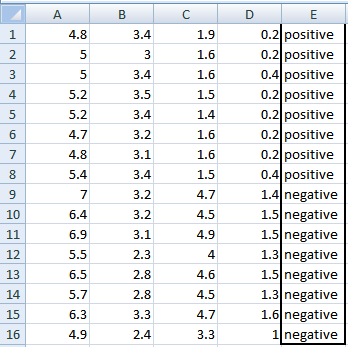
\includegraphics[width=3.62in,height=3.62in]{./media/image1.png}
	\end{Center}
\end{figure}


%%%%%%%%%%%%%%%%%%%% Figure/Image No: 1 Ends here %%%%%%%%%%%%%%%%%%%%

\par

{\fontsize{11pt}{13.2pt}\selectfont A, B, C, D attributes can be considered as predictors \par}\par

{\fontsize{11pt}{13.2pt}\selectfont E column class labels can be considered as a target variable. \par}\par

{\fontsize{11pt}{13.2pt}\selectfont For constructing a decision tree from this data, we have to convert continuous data into categorical data.\par}\par

{\fontsize{11pt}{13.2pt}\selectfont Categorization is done by,\par}\par

A:\  >=5 or <5\par

B:\  >=3 or <3\par

C:\  >=4.2 or <4.2\par

D:\  >=1.4 or <1.4\par

Entropy used for finding IG is given by,\par



%%%%%%%%%%%%%%%%%%%% Figure/Image No: 2 starts here %%%%%%%%%%%%%%%%%%%%

\begin{figure}[H]
	\begin{Center}
		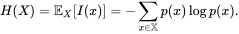
\includegraphics[width=2.49in,height=0.35in]{./media/image2.png}
	\end{Center}
\end{figure}


%%%%%%%%%%%%%%%%%%%% Figure/Image No: 2 Ends here %%%%%%%%%%%%%%%%%%%%

\par

Now calculating IG for A, \par

\setlength{\parskip}{5.04pt}
Var A has value >=5 for 12 records out of 16 and 4 records with value <5 value.\par

(A >= 5 and class is positive): 5/12\par

(A >= 5 and class is negative): 7/12\par

 \[ Entropy \left( 5,7 \right)  = -1 \ast  \left(   \left( 5/12 \right) \astlog2 \left( 5/12 \right)  +  \left( 7/12 \right) \astlog2 \left( 7/12 \right)  \right)  = 0.9799 \] \par

(A <5 and class is positive): ¾\par

(A <5 and class is negative): ¼\par

 \[ Entropy \left( 3,1 \right)  =  -1 \ast  \left(   \left( 3/4 \right) \astlog2 \left( 3/4 \right)  +  \left( 1/4 \right) \astlog2 \left( 1/4 \right)  \right)  = 0.81128 \] \par

 \[ Entropy \left( Target, A \right)  = P \left( >=5 \right)  \ast E \left( 5,7 \right)  + P \left( <5 \right)  \ast E \left( 3,1 \right) =  \left( 12/16 \right)  \ast 0.9799 +  \left( 4/16 \right)  \ast 0.81128 = 0.937745 \] \par

Information Gain for A = E(Target) – E(Target, A) = 1 – 0.937745 = 0.062255\par

Similarly, \par

IG(A) = 0.062255\par

IG(B) = 0.707095\par

IG(C) = 0.5488\par

IG(D) = 0.41189\par

Using IG values in descending order we can construct DT as,\par


\vspace{\baselineskip}
\vspace{\baselineskip}

\vspace{\baselineskip}
\begin{Center}
{\fontsize{18pt}{21.6pt}\selectfont b) Naive Bayesian Classifier (NBC)\par}
\end{Center}\par


\vspace{\baselineskip}
{\fontsize{14pt}{16.8pt}\selectfont Read about Bayes theorem, conditional class independence, prior and posterior probabilities.\par}\par

{\fontsize{14pt}{16.8pt}\selectfont How to handle zero probability scenario (Laplacian Estimator)\par}\par

{\fontsize{14pt}{16.8pt}\selectfont Give a short pseudo code and trace.\par}\par

{\fontsize{14pt}{16.8pt}\selectfont \uline{Pseudo Code}\par}\par

Target Variable – Y (true or false -- binary)\par

Predictor Variables – X1 .. Xn\par

\begin{enumerate}
	\item From the data, Estimate P(Y = true) and P(Y = false)\par

	\item To do (1), For every value xij of each input attribute Xi, \par

\begin{enumerate}
	\item Find P(Xi = xij $ \vert $  Y = true)\par

	\item Find P(Xi = xij $ \vert $  Y = false)
\end{enumerate}
\end{enumerate}\par

Now, Classify a new X’ by, \par

(Let PROD(true) = $ \{ $ P(X1$ \vert $ Y=true). P(X2$ \vert $ Y=true)$ \ldots $ P(Xn$ \vert $ Y=true)$ \} $ )\par

(Let PROD(false) = $ \{ $ P(X1$ \vert $ Y= false). P(X2$ \vert $ Y= false)$ \ldots $ P(Xn$ \vert $ Y= false)$ \} $ )\par

Y’ (Predicted Class for X’) = \par

True if P(Y = true)PROD(true) > P(Y = false)PROD(false)\par

False if P(Y = true)PROD(true) <= P(Y = false)PROD(false)\par

{\fontsize{14pt}{16.8pt}\selectfont \uline{Trace}\par}\par



%%%%%%%%%%%%%%%%%%%% Table No: 1 starts here %%%%%%%%%%%%%%%%%%%%


\begin{table}[H]
 			\centering
\begin{tabular}{p{0.31in}p{0.54in}p{0.81in}p{0.5in}p{0.36in}p{0.28in}}
\hline
%row no:1
\multicolumn{1}{p{0.31in}}{\Centering {\fontsize{8pt}{9.6pt}\selectfont \textbf{\uppercase{INDEX}}}} & 
\multicolumn{1}{p{0.54in}}{\Centering {\fontsize{8pt}{9.6pt}\selectfont \textbf{\uppercase{OUTLOOK}}}} & 
\multicolumn{1}{p{0.81in}}{\Centering {\fontsize{8pt}{9.6pt}\selectfont \textbf{\uppercase{TEMPERATURE}}}} & 
\multicolumn{1}{p{0.5in}}{\Centering {\fontsize{8pt}{9.6pt}\selectfont \textbf{\uppercase{HUMIDITY}}}} & 
\multicolumn{1}{p{0.36in}}{\Centering {\fontsize{8pt}{9.6pt}\selectfont \textbf{\uppercase{WINDY}}}} & 

\hhline{~~~~~}
%row no:2
\multicolumn{1}{p{0.31in}}{\Centering {\fontsize{8pt}{9.6pt}\selectfont 0}} & 
\multicolumn{1}{p{0.54in}}{\Centering {\fontsize{8pt}{9.6pt}\selectfont Rainy}} & 
\multicolumn{1}{p{0.81in}}{\Centering {\fontsize{8pt}{9.6pt}\selectfont Hot}} & 
\multicolumn{1}{p{0.5in}}{\Centering {\fontsize{8pt}{9.6pt}\selectfont High}} & 
\multicolumn{1}{p{0.36in}}{\Centering {\fontsize{8pt}{9.6pt}\selectfont False}} & 
\multicolumn{1}{p{0.28in}}{\Centering {\fontsize{8pt}{9.6pt}\selectfont No}} \\
\hhline{~~~~~~}
%row no:3
\multicolumn{1}{p{0.31in}}{\Centering {\fontsize{8pt}{9.6pt}\selectfont 1}} & 
\multicolumn{1}{p{0.54in}}{\Centering {\fontsize{8pt}{9.6pt}\selectfont Rainy}} & 
\multicolumn{1}{p{0.81in}}{\Centering {\fontsize{8pt}{9.6pt}\selectfont Hot}} & 
\multicolumn{1}{p{0.5in}}{\Centering {\fontsize{8pt}{9.6pt}\selectfont High}} & 
\multicolumn{1}{p{0.36in}}{\Centering {\fontsize{8pt}{9.6pt}\selectfont True}} & 
\multicolumn{1}{p{0.28in}}{\Centering {\fontsize{8pt}{9.6pt}\selectfont No}} \\
\hhline{~~~~~~}
%row no:4
\multicolumn{1}{p{0.31in}}{\Centering {\fontsize{8pt}{9.6pt}\selectfont 2}} & 
\multicolumn{1}{p{0.54in}}{\Centering {\fontsize{8pt}{9.6pt}\selectfont Overcast}} & 
\multicolumn{1}{p{0.81in}}{\Centering {\fontsize{8pt}{9.6pt}\selectfont Hot}} & 
\multicolumn{1}{p{0.5in}}{\Centering {\fontsize{8pt}{9.6pt}\selectfont High}} & 
\multicolumn{1}{p{0.36in}}{\Centering {\fontsize{8pt}{9.6pt}\selectfont False}} & 
\multicolumn{1}{p{0.28in}}{\Centering {\fontsize{8pt}{9.6pt}\selectfont Yes}} \\
\hhline{~~~~~~}
%row no:5
\multicolumn{1}{p{0.31in}}{\Centering {\fontsize{8pt}{9.6pt}\selectfont 3}} & 
\multicolumn{1}{p{0.54in}}{\Centering {\fontsize{8pt}{9.6pt}\selectfont Sunny}} & 
\multicolumn{1}{p{0.81in}}{\Centering {\fontsize{8pt}{9.6pt}\selectfont Mild}} & 
\multicolumn{1}{p{0.5in}}{\Centering {\fontsize{8pt}{9.6pt}\selectfont High}} & 
\multicolumn{1}{p{0.36in}}{\Centering {\fontsize{8pt}{9.6pt}\selectfont False}} & 
\multicolumn{1}{p{0.28in}}{\Centering {\fontsize{8pt}{9.6pt}\selectfont Yes}} \\
\hhline{~~~~~~}
%row no:6
\multicolumn{1}{p{0.31in}}{\Centering {\fontsize{8pt}{9.6pt}\selectfont 4}} & 
\multicolumn{1}{p{0.54in}}{\Centering {\fontsize{8pt}{9.6pt}\selectfont Sunny}} & 
\multicolumn{1}{p{0.81in}}{\Centering {\fontsize{8pt}{9.6pt}\selectfont Cool}} & 
\multicolumn{1}{p{0.5in}}{\Centering {\fontsize{8pt}{9.6pt}\selectfont Normal}} & 
\multicolumn{1}{p{0.36in}}{\Centering {\fontsize{8pt}{9.6pt}\selectfont False}} & 
\multicolumn{1}{p{0.28in}}{\Centering {\fontsize{8pt}{9.6pt}\selectfont Yes}} \\
\hhline{~~~~~~}
%row no:7
\multicolumn{1}{p{0.31in}}{\Centering {\fontsize{8pt}{9.6pt}\selectfont 5}} & 
\multicolumn{1}{p{0.54in}}{\Centering {\fontsize{8pt}{9.6pt}\selectfont Sunny}} & 
\multicolumn{1}{p{0.81in}}{\Centering {\fontsize{8pt}{9.6pt}\selectfont Cool}} & 
\multicolumn{1}{p{0.5in}}{\Centering {\fontsize{8pt}{9.6pt}\selectfont Normal}} & 
\multicolumn{1}{p{0.36in}}{\Centering {\fontsize{8pt}{9.6pt}\selectfont True}} & 
\multicolumn{1}{p{0.28in}}{\Centering {\fontsize{8pt}{9.6pt}\selectfont No}} \\
\hhline{~~~~~~}
%row no:8
\multicolumn{1}{p{0.31in}}{\Centering {\fontsize{8pt}{9.6pt}\selectfont 6}} & 
\multicolumn{1}{p{0.54in}}{\Centering {\fontsize{8pt}{9.6pt}\selectfont Overcast}} & 
\multicolumn{1}{p{0.81in}}{\Centering {\fontsize{8pt}{9.6pt}\selectfont Cool}} & 
\multicolumn{1}{p{0.5in}}{\Centering {\fontsize{8pt}{9.6pt}\selectfont Normal}} & 
\multicolumn{1}{p{0.36in}}{\Centering {\fontsize{8pt}{9.6pt}\selectfont True}} & 
\multicolumn{1}{p{0.28in}}{\Centering {\fontsize{8pt}{9.6pt}\selectfont Yes}} \\
\hhline{~~~~~~}
%row no:9
\multicolumn{1}{p{0.31in}}{\Centering {\fontsize{8pt}{9.6pt}\selectfont 7}} & 
\multicolumn{1}{p{0.54in}}{\Centering {\fontsize{8pt}{9.6pt}\selectfont Rainy}} & 
\multicolumn{1}{p{0.81in}}{\Centering {\fontsize{8pt}{9.6pt}\selectfont Mild}} & 
\multicolumn{1}{p{0.5in}}{\Centering {\fontsize{8pt}{9.6pt}\selectfont High}} & 
\multicolumn{1}{p{0.36in}}{\Centering {\fontsize{8pt}{9.6pt}\selectfont False}} & 
\multicolumn{1}{p{0.28in}}{\Centering {\fontsize{8pt}{9.6pt}\selectfont No}} \\
\hhline{~~~~~~}
%row no:10
\multicolumn{1}{p{0.31in}}{\Centering {\fontsize{8pt}{9.6pt}\selectfont 8}} & 
\multicolumn{1}{p{0.54in}}{\Centering {\fontsize{8pt}{9.6pt}\selectfont Rainy}} & 
\multicolumn{1}{p{0.81in}}{\Centering {\fontsize{8pt}{9.6pt}\selectfont Cool}} & 
\multicolumn{1}{p{0.5in}}{\Centering {\fontsize{8pt}{9.6pt}\selectfont Normal}} & 
\multicolumn{1}{p{0.36in}}{\Centering {\fontsize{8pt}{9.6pt}\selectfont False}} & 
\multicolumn{1}{p{0.28in}}{\Centering {\fontsize{8pt}{9.6pt}\selectfont Yes}} \\
\hhline{~~~~~~}
%row no:11
\multicolumn{1}{p{0.31in}}{\Centering {\fontsize{8pt}{9.6pt}\selectfont 9}} & 
\multicolumn{1}{p{0.54in}}{\Centering {\fontsize{8pt}{9.6pt}\selectfont Sunny}} & 
\multicolumn{1}{p{0.81in}}{\Centering {\fontsize{8pt}{9.6pt}\selectfont Mild}} & 
\multicolumn{1}{p{0.5in}}{\Centering {\fontsize{8pt}{9.6pt}\selectfont Normal}} & 
\multicolumn{1}{p{0.36in}}{\Centering {\fontsize{8pt}{9.6pt}\selectfont False}} & 
\multicolumn{1}{p{0.28in}}{\Centering {\fontsize{8pt}{9.6pt}\selectfont Yes}} \\
\hhline{~~~~~~}
%row no:12
\multicolumn{1}{p{0.31in}}{\Centering {\fontsize{8pt}{9.6pt}\selectfont 10}} & 
\multicolumn{1}{p{0.54in}}{\Centering {\fontsize{8pt}{9.6pt}\selectfont Rainy}} & 
\multicolumn{1}{p{0.81in}}{\Centering {\fontsize{8pt}{9.6pt}\selectfont Mild}} & 
\multicolumn{1}{p{0.5in}}{\Centering {\fontsize{8pt}{9.6pt}\selectfont Normal}} & 
\multicolumn{1}{p{0.36in}}{\Centering {\fontsize{8pt}{9.6pt}\selectfont True}} & 
\multicolumn{1}{p{0.28in}}{\Centering {\fontsize{8pt}{9.6pt}\selectfont Yes}} \\
\hhline{~~~~~~}
%row no:13
\multicolumn{1}{p{0.31in}}{\Centering {\fontsize{8pt}{9.6pt}\selectfont 11}} & 
\multicolumn{1}{p{0.54in}}{\Centering {\fontsize{8pt}{9.6pt}\selectfont Overcast}} & 
\multicolumn{1}{p{0.81in}}{\Centering {\fontsize{8pt}{9.6pt}\selectfont Mild}} & 
\multicolumn{1}{p{0.5in}}{\Centering {\fontsize{8pt}{9.6pt}\selectfont High}} & 
\multicolumn{1}{p{0.36in}}{\Centering {\fontsize{8pt}{9.6pt}\selectfont True}} & 
\multicolumn{1}{p{0.28in}}{\Centering {\fontsize{8pt}{9.6pt}\selectfont Yes}} \\
\hhline{~~~~~~}
%row no:14
\multicolumn{1}{p{0.31in}}{\Centering {\fontsize{8pt}{9.6pt}\selectfont 12}} & 
\multicolumn{1}{p{0.54in}}{\Centering {\fontsize{8pt}{9.6pt}\selectfont Overcast}} & 
\multicolumn{1}{p{0.81in}}{\Centering {\fontsize{8pt}{9.6pt}\selectfont Hot}} & 
\multicolumn{1}{p{0.5in}}{\Centering {\fontsize{8pt}{9.6pt}\selectfont Normal}} & 
\multicolumn{1}{p{0.36in}}{\Centering {\fontsize{8pt}{9.6pt}\selectfont False}} & 
\multicolumn{1}{p{0.28in}}{\Centering {\fontsize{8pt}{9.6pt}\selectfont Yes}} \\
\hhline{~~~~~~}
%row no:15
\multicolumn{1}{p{0.31in}}{\Centering {\fontsize{8pt}{9.6pt}\selectfont 13}} & 
\multicolumn{1}{p{0.54in}}{\Centering {\fontsize{8pt}{9.6pt}\selectfont Sunny}} & 
\multicolumn{1}{p{0.81in}}{\Centering {\fontsize{8pt}{9.6pt}\selectfont Mild}} & 
\multicolumn{1}{p{0.5in}}{\Centering {\fontsize{8pt}{9.6pt}\selectfont High}} & 
\multicolumn{1}{p{0.36in}}{\Centering {\fontsize{8pt}{9.6pt}\selectfont True}} & 
\multicolumn{1}{p{0.28in}}{\Centering {\fontsize{8pt}{9.6pt}\selectfont No}} \\
\hhline{~~~~~~}

\end{tabular}
 \end{table}


%%%%%%%%%%%%%%%%%%%% Table No: 1 ends here %%%%%%%%%%%%%%%%%%%%

We assume that all attributes are independent and are of equal importance to outcome.\par

Then we find P(Xi=xij$ \vert $ Y=Yes) and P(Xi=xij$ \vert $ Y=No)\par



%%%%%%%%%%%%%%%%%%%% Figure/Image No: 3 starts here %%%%%%%%%%%%%%%%%%%%

\begin{figure}[H]
	\begin{Center}
		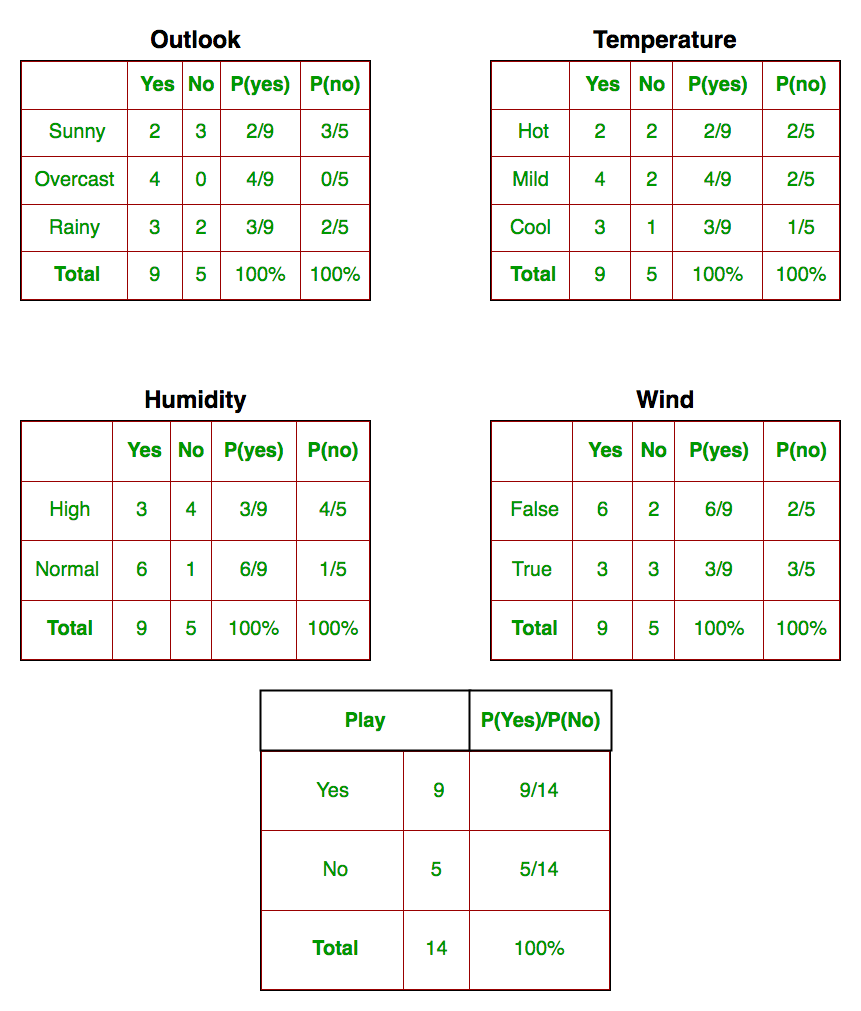
\includegraphics[width=6.5in,height=6.5in]{./media/image3.png}
	\end{Center}
\end{figure}


%%%%%%%%%%%%%%%%%%%% Figure/Image No: 3 Ends here %%%%%%%%%%%%%%%%%%%%

\par

Now that we have this data, \par

Suppose test data is \par

Today = (Sunny, Hot, Normal, False)\par

By Bayes Theorem, \par

 \[ P \left( Yes \vert today \right)  = \frac{P \left( Sunny \vert Yes \right)  P \left( Hot \vert Yes \right)  P \left( Normal \vert Yes \right)  P \left( False \vert Yes \right)  P \left( Yes \right)  }{P \left( today \right) } \] \par

=  \( \frac{\frac{2}{9}~.~~\frac{2}{9}~.~~\frac{6}{9}~.~~\frac{6}{9}~.~~\frac{9}{14}}{P \left( today \right) } \)  =  \( \frac{0.0141}{P \left( today \right) } \) \par

 \[ P \left( No \vert today \right)  = \frac{P \left( Sunny \vert No \right)  P \left( Hot \vert No \right)  P \left( Normal \vert No \right)  P \left( False \vert No \right)  P \left( No \right)  }{P \left( today \right) } \] \par

=  \( \frac{\frac{3}{5}~.~~\frac{2}{5}~.~~\frac{1}{5}~.~~\frac{2}{5}~.~~\frac{5}{14}}{P \left( today \right) } \)  =  \( \frac{0.0068}{P \left( today \right) } \) \par

As P(today) > 0, \par

Clearly P(Yes) > P(No)\par

So, predicted value for playing golf is YES.\par


\vspace{\baselineskip}
For Problems with Zero Probability, use\par

Laplace smoothing: By applying this method, prior probability and conditional probability are, K is the number of different values in y and A is the number of different values in aj.\par


\vspace{\baselineskip}
\begin{Center}
{\fontsize{18pt}{21.6pt}\selectfont c) Neural Network Classifier (Back Propagation Network(BPN))\par}
\end{Center}\par


\vspace{\baselineskip}
{\fontsize{14pt}{16.8pt}\selectfont Understand basic terminologies - topology of a network, input layer, hidden layer, output layer, activation functions, weight, bias.\par}\par

{\fontsize{14pt}{16.8pt}\selectfont Strength and limitations of a neural network.\par}\par

{\fontsize{14pt}{16.8pt}\selectfont Take a sample network to learn the basics. For instance, learning the behaviour of OR gate, AND gate.\par}\par

{\fontsize{14pt}{16.8pt}\selectfont Take a network involving atleast one hidden layer and trace the BPN algorithm assuming a target class for one epoch.\par}\par


\vspace{\baselineskip}

\vspace{\baselineskip}
{\fontsize{14pt}{16.8pt}\selectfont \uline{Trace}\par}\par

Example Dataset \par



%%%%%%%%%%%%%%%%%%%% Table No: 2 starts here %%%%%%%%%%%%%%%%%%%%


\begin{table}[H]
 			\centering
\begin{tabular}{p{1.96in}p{1.96in}p{1.96in}}
\hline
%row no:1
\multicolumn{1}{|p{1.96in}}{Class} & 
\multicolumn{1}{|p{1.96in}}{x} & 
\multicolumn{1}{|p{1.96in}|}{y} \\
\hhline{---}
%row no:2
\multicolumn{1}{|p{1.96in}}{class 1 (w1)} & 
\multicolumn{1}{|p{1.96in}}{2} & 
\multicolumn{1}{|p{1.96in}|}{2} \\
\hhline{---}
%row no:3
\multicolumn{1}{|p{1.96in}}{class 1 (w1)} & 
\multicolumn{1}{|p{1.96in}}{-1} & 
\multicolumn{1}{|p{1.96in}|}{2} \\
\hhline{---}
%row no:4
\multicolumn{1}{|p{1.96in}}{class 1 (w1)} & 
\multicolumn{1}{|p{1.96in}}{1} & 
\multicolumn{1}{|p{1.96in}|}{3} \\
\hhline{---}
%row no:5
\multicolumn{1}{|p{1.96in}}{class 1 (w1)} & 
\multicolumn{1}{|p{1.96in}}{-1} & 
\multicolumn{1}{|p{1.96in}|}{-1} \\
\hhline{---}
%row no:6
\multicolumn{1}{|p{1.96in}}{class 1 (w1)} & 
\multicolumn{1}{|p{1.96in}}{0.5} & 
\multicolumn{1}{|p{1.96in}|}{0.5} \\
\hhline{---}
%row no:7
\multicolumn{1}{|p{1.96in}}{class 2 (w2)} & 
\multicolumn{1}{|p{1.96in}}{-1} & 
\multicolumn{1}{|p{1.96in}|}{-3} \\
\hhline{---}
%row no:8
\multicolumn{1}{|p{1.96in}}{class 2 (w2)} & 
\multicolumn{1}{|p{1.96in}}{0} & 
\multicolumn{1}{|p{1.96in}|}{-1} \\
\hhline{---}
%row no:9
\multicolumn{1}{|p{1.96in}}{class 2 (w2)} & 
\multicolumn{1}{|p{1.96in}}{1} & 
\multicolumn{1}{|p{1.96in}|}{-2} \\
\hhline{---}
%row no:10
\multicolumn{1}{|p{1.96in}}{class 2 (w2)} & 
\multicolumn{1}{|p{1.96in}}{-1} & 
\multicolumn{1}{|p{1.96in}|}{-2} \\
\hhline{---}
%row no:11
\multicolumn{1}{|p{1.96in}}{class 2 (w2)} & 
\multicolumn{1}{|p{1.96in}}{0} & 
\multicolumn{1}{|p{1.96in}|}{-2} \\
\hhline{---}

\end{tabular}
 \end{table}


%%%%%%%%%%%%%%%%%%%% Table No: 2 ends here %%%%%%%%%%%%%%%%%%%%


\vspace{\baselineskip}
We take a neural network with 3 layers\par

\begin{enumerate}
	\item 1 – input layer (2 nodes + 1 bias)\par

	\item 1 – hidden layer (2 nodes + 1 bias)\par

	\item 1 – output layer (2 nodes)
\end{enumerate}\par

Hyperparameters are taken as,\par

\begin{enumerate}
	\item Learning Rate = 0.5\par

	\item Activation Function – Sigmoid \par

	\item Epochs = 1000\par

	\item Weights = Random
\end{enumerate}\par

Now, for forward propagation,\par

Value at a node is given by, \par

 \[ N_{k}^{i+1}~= f \left(  \sum _{j+1}^{n} \left( W_{jk}^{i}\ast N_{j}^{i} \right)  \right)  \] \par

 \( N_{k}^{i+1} \)  is the i+1 th node in k th layer (it also includes the bias node). \par

n is the total number of nodes in i th layer. \par

f(.) is the activation function.\par

Therefore, if we use the above formula, we get, \par

 \( N_{1}^{1} \) \  (H1) = f(W\textsuperscript{1}11 $\ast$  x + W\textsuperscript{1}21 $\ast$  y + W\textsuperscript{1}31 $\ast$  1) \par

 \( N_{2}^{1} \)  (H2) = f(W\textsuperscript{1}12 $\ast$  x + W\textsuperscript{1}22 $\ast$  y + W\textsuperscript{1}32 $\ast$  1) \par

 \( N_{1}^{2} \)  (O1) = f(W\textsuperscript{2}11 $\ast$  H1 + W\textsuperscript{2}21 $\ast$  H2 + W\textsuperscript{2}31 $\ast$  1) \par

 \( N_{2}^{2} \)  (O2) = f(W\textsuperscript{2}12 $\ast$  H1 + W\textsuperscript{2}22 $\ast$  H2 + W\textsuperscript{2}32 $\ast$  1) \par

When we plug in the values for the first value of the dataset i.e. (2, 2), We get, \par

H1 = f(0.13436424411240122 $\ast$  2 + 0.8474337369372327 $\ast$  2 + 0.763774618976614 $\ast$  1) =f(2.7273705810758817) = 0.9386225302230806 \par

H2 = f(0.2550690257394217 $\ast$  2 + 0.49543508709194095 $\ast$  2 + 0.4494910647887381 $\ast$  1) = f(1.9504992904514635) = 0.8755010741482664 \par

O1 = f(0.651592972722763 $\ast$  0.9386225302230806 + 0.7887233511355132 $\ast$  0.8755010741482664 + 0.0938595867742349 $\ast$  1) = f(1.3959875726318156) = 0.8015464048450159 29 B ANIRUDH \par

O2 = f(0.02834747652200631 $\ast$  0.9386225302230806 + 0.8357651039198697 $\ast$  0.8755010741482664 + 0.43276706790505337 $\ast$  1) = f(1.1910878942610617) = 0.7669355767878618\par

Next is backpropagation of the error,\par

\begin{enumerate}
	\item For a unit j in the output layer, the error Err\textsubscript{j} is computed by, \par

 \[ Errj~= Outj  \left( 1 - Outj~ \right)  \ast  \left( Tj~-~Outj  \right)  \] \par

Out\textsubscript{j} (1 - Out\textsubscript{j} ) is the derivative of the logistic (sigmoid) function. \par

T\textsubscript{j }is the target value of the O\textsubscript{j} node.\par

	\item In hidden layer,
\end{enumerate}\par

 \[ Errj~= Outj  \left( 1 - Outj~ \right)  \ast~ \sum _{k}^{}Err_{k}~\ast~W_{jk}~ \] \par


\vspace{\baselineskip}
\tab  \( W_{jk} \)  is the weight of the connection from unit j to a unit k in the next higher layer. \par

 \( Err_{k}~ \) is the is the error of unit k.\par

The weights and biases are updated to reflect the propagated errors. Weights are updated by the following equations, where $ \Delta $   \( W_{ij} \)  is the change in weight  \( W_{ij} \) :\par

 \[  \Delta W_{ij} =  \left( l \right) \astErrj \ast~Outi~ \] \par

 \[ W_{ij}= W_{ij} +  \Delta W_{ij} \] \par

(l – learning rate)\par

So, the error for Err1 for the output layer is, \par

Erri = 0.8015464048450159 $\ast$  (1 - 0.8015464048450159) $\ast$  (1 - 0.8015464048450159) = 0.03156796688859639 \par

The change in weight for Hidden Layer is, \par

$ \Delta $  W11 = (0.5) $\ast$  (0.03156796688859639) $\ast$  (0.9386225302230806) = 0.014815202477486385 \par

W11 = 0.651592972722763 + 0.014815202477486385 = 0.6664081752002493 \par

Similarly, the error for Err1 for the Hidden Layer is, \par

Erri = 0.9386225302230806 $\ast$  (1 - 0.9386225302230806) $\ast$  (0.03156796688859639 $\ast$  0.651592972722763 + (0.7669355767878618) $\ast$  (1 - 0.7669355767878618) $\ast$  (0 - 0.7669355767878618) $\ast$  0.02834747652200631) = 0.0009611362816286504 \par

The change in weight for Hidden Layer is, \par

$ \Delta $  W11 = (0.5) $\ast$  (0.0009611362816286504) $\ast$  (2) = 0.0009611362816286504 \par

W11 = 0.13436424411240122 + 0.0009611362816286504 = 0.13532538039402986\par

Now, again forward propagate and backpropagate and update weights and repeat.\par


\vspace{\baselineskip}
\begin{Center}
{\fontsize{18pt}{21.6pt}\selectfont d) SVM or Nearest Neighbour Classifier (Anyone)\par}
\end{Center}\par


\vspace{\baselineskip}
{\fontsize{14pt}{16.8pt}\selectfont Understand the algorithm/working and give the pseudocode and the trace\par}\par

{\fontsize{14pt}{16.8pt}\selectfont \uline{Pseudo Code}\par}\par

k-Nearest Neighbour\par

Classify (X, Y, x) where X: training data, Y: class labels of X, x: test sample\par

For i = 1 to m do\par

\tab Computer distance d(Xi, x)\par

End for\par

Computer set I containing indices for the k smallest distances d(Xi, x)\par

Return majority label for $ \{ $ Yi where i \textcolor[HTML]{222222}{$ \in $  I}$ \} $ \par

{\fontsize{14pt}{16.8pt}\selectfont \uline{Trace}\par}\par

Consider binary Y with attributes X\par

\textbf{K = 3}\par



%%%%%%%%%%%%%%%%%%%% Table No: 3 starts here %%%%%%%%%%%%%%%%%%%%


\begin{table}[H]
 			\centering
\begin{tabular}{p{1.94in}p{1.9in}p{2.05in}}
\hline
%row no:1
\multicolumn{1}{|p{1.94in}}{\Centering X1} & 
\multicolumn{1}{|p{1.9in}}{\Centering X2} & 
\multicolumn{1}{|p{2.05in}|}{\Centering Y} \\
\hhline{---}
%row no:2
\multicolumn{1}{|p{1.94in}}{\Centering 1} & 
\multicolumn{1}{|p{1.9in}}{\Centering 2} & 
\multicolumn{1}{|p{2.05in}|}{\Centering False} \\
\hhline{---}
%row no:3
\multicolumn{1}{|p{1.94in}}{\Centering 2} & 
\multicolumn{1}{|p{1.9in}}{\Centering 3} & 
\multicolumn{1}{|p{2.05in}|}{\Centering True} \\
\hhline{---}
%row no:4
\multicolumn{1}{|p{1.94in}}{\Centering 3} & 
\multicolumn{1}{|p{1.9in}}{\Centering 1} & 
\multicolumn{1}{|p{2.05in}|}{\Centering True} \\
\hhline{---}
%row no:5
\multicolumn{1}{|p{1.94in}}{\Centering 4} & 
\multicolumn{1}{|p{1.9in}}{\Centering 3} & 
\multicolumn{1}{|p{2.05in}|}{\Centering False} \\
\hhline{---}
%row no:6
\multicolumn{1}{|p{1.94in}}{\Centering 5} & 
\multicolumn{1}{|p{1.9in}}{\Centering 5} & 
\multicolumn{1}{|p{2.05in}|}{\Centering False} \\
\hhline{---}
%row no:7
\multicolumn{1}{|p{1.94in}}{\Centering 6} & 
\multicolumn{1}{|p{1.9in}}{\Centering 1} & 
\multicolumn{1}{|p{2.05in}|}{\Centering False} \\
\hhline{---}
%row no:8
\multicolumn{1}{|p{1.94in}}{\Centering 7} & 
\multicolumn{1}{|p{1.9in}}{\Centering 2} & 
\multicolumn{1}{|p{2.05in}|}{\Centering True} \\
\hhline{---}

\end{tabular}
 \end{table}


%%%%%%%%%%%%%%%%%%%% Table No: 3 ends here %%%%%%%%%%%%%%%%%%%%


\vspace{\baselineskip}
Now for a test x = (2.5, 3.5), \par

D(X,\ x) =>   \( \sqrt[]{ \left( X1-x1 \right) ^{2}+  \left( X2-x2 \right) ^{2}} \) \par



%%%%%%%%%%%%%%%%%%%% Table No: 4 starts here %%%%%%%%%%%%%%%%%%%%


\begin{table}[H]
 			\centering
\begin{tabular}{p{1.94in}p{1.9in}p{2.05in}}
\hline
%row no:1
\multicolumn{1}{|p{1.94in}}{\Centering X1} & 
\multicolumn{1}{|p{1.9in}}{\Centering X2} & 
\multicolumn{1}{|p{2.05in}|}{\Centering D(X, x)} \\
\hhline{---}
%row no:2
\multicolumn{1}{|p{1.94in}}{\Centering 1} & 
\multicolumn{1}{|p{1.9in}}{\Centering 2} & 
\multicolumn{1}{|p{2.05in}|}{\Centering 2.12} \\
\hhline{---}
%row no:3
\multicolumn{1}{|p{1.94in}}{\Centering 2} & 
\multicolumn{1}{|p{1.9in}}{\Centering 3} & 
\multicolumn{1}{|p{2.05in}|}{\Centering 0.71} \\
\hhline{---}
%row no:4
\multicolumn{1}{|p{1.94in}}{\Centering 3} & 
\multicolumn{1}{|p{1.9in}}{\Centering 1} & 
\multicolumn{1}{|p{2.05in}|}{\Centering 2.55} \\
\hhline{---}
%row no:5
\multicolumn{1}{|p{1.94in}}{\Centering 4} & 
\multicolumn{1}{|p{1.9in}}{\Centering 3} & 
\multicolumn{1}{|p{2.05in}|}{\Centering 1.58} \\
\hhline{---}
%row no:6
\multicolumn{1}{|p{1.94in}}{\Centering 5} & 
\multicolumn{1}{|p{1.9in}}{\Centering 5} & 
\multicolumn{1}{|p{2.05in}|}{\Centering 2.91} \\
\hhline{---}
%row no:7
\multicolumn{1}{|p{1.94in}}{\Centering 6} & 
\multicolumn{1}{|p{1.9in}}{\Centering 1} & 
\multicolumn{1}{|p{2.05in}|}{\Centering 4.30} \\
\hhline{---}
%row no:8
\multicolumn{1}{|p{1.94in}}{\Centering 7} & 
\multicolumn{1}{|p{1.9in}}{\Centering 2} & 
\multicolumn{1}{|p{2.05in}|}{\Centering 4.74} \\
\hhline{---}

\end{tabular}
 \end{table}


%%%%%%%%%%%%%%%%%%%% Table No: 4 ends here %%%%%%%%%%%%%%%%%%%%


\vspace{\baselineskip}
As K = 3, minimum 3 distances is for (2, 3), (4, 3), (1, 2)\par

And their Y is True, False, False\par

SO, majority is FALSE = y for x\par


\vspace{\baselineskip}

\vspace{\baselineskip}

\vspace{\baselineskip}

\vspace{\baselineskip}

\vspace{\baselineskip}

\vspace{\baselineskip}

\vspace{\baselineskip}

\vspace{\baselineskip}

\vspace{\baselineskip}

\vspace{\baselineskip}
\begin{Center}
{\fontsize{28pt}{33.6pt}\selectfont Q II\par}
\end{Center}\par

{\fontsize{14pt}{16.8pt}\selectfont II) Understand the working of a simple genetic algorithm involving operators of selection, cross-over, mutation. Apply these operators to an optimisation function such as max f(x)= x3-2x2+x within a range of (0,31).\par}\par

{\fontsize{14pt}{16.8pt}\selectfont (Refer David E. Goldberg material for basics of GA)\par}\par


\vspace{\baselineskip}
{\fontsize{14pt}{16.8pt}\selectfont Code in GeneticOptimisation.py under Codes Folder\par}\par

{\fontsize{14pt}{16.8pt}\selectfont Run for\par}\par

\setlength{\parskip}{0.0pt}
{\fontsize{10pt}{12.0pt}\selectfont \textcolor[HTML]{D4D4D4}{sol\_per\_pop = 200 $\#$  Defining the population size.}\par}\par

{\fontsize{10pt}{12.0pt}\selectfont \textcolor[HTML]{D4D4D4}{num\_generations = 5000}\par}\par

{\fontsize{10pt}{12.0pt}\selectfont \textcolor[HTML]{D4D4D4}{num\_parents\_mating = 100}\par}\par

{\fontsize{10pt}{12.0pt}\selectfont \textcolor[HTML]{D4D4D4}{select\_mating\_pool = select\_mating\_pool\_bestfitness}\par}\par

{\fontsize{10pt}{12.0pt}\selectfont \textcolor[HTML]{D4D4D4}{crossover = crossover\_OnePoint}\par}\par

{\fontsize{10pt}{12.0pt}\selectfont \textcolor[HTML]{D4D4D4}{mutation = mutation\_UniformNoise}\par}\par

{\fontsize{10pt}{12.0pt}\selectfont \textcolor[HTML]{D4D4D4}{fitness\_func = PolynomialFitness}\par}\par

{\fontsize{10pt}{12.0pt}\selectfont \textcolor[HTML]{D4D4D4}{boundary = (0, 31)}\par}\par

{\fontsize{10pt}{12.0pt}\selectfont \textcolor[HTML]{D4D4D4}{equation\_inputs = [0, -2, 1]}\par}\par

{\fontsize{10pt}{12.0pt}\selectfont \textcolor[HTML]{D4D4D4}{num\_weights = 1 $\#$  Number of the weights we are looking to optimize.}\par}\par


\vspace{\baselineskip}
{\fontsize{14pt}{16.8pt}\selectfont Output:\par}\par

Fitness Graph\par



%%%%%%%%%%%%%%%%%%%% Figure/Image No: 4 starts here %%%%%%%%%%%%%%%%%%%%

\begin{figure}[H]
	\begin{Center}
		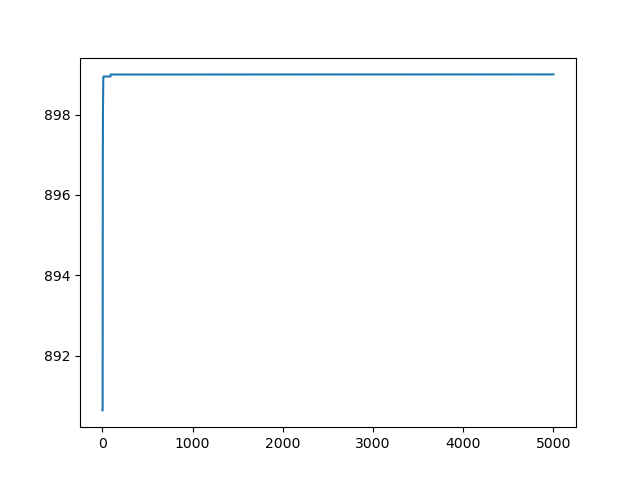
\includegraphics[width=3.16in,height=2.37in]{./media/image4.png}
	\end{Center}
\end{figure}


%%%%%%%%%%%%%%%%%%%% Figure/Image No: 4 Ends here %%%%%%%%%%%%%%%%%%%%

\par


\vspace{\baselineskip}

\vspace{\baselineskip}
Gene Updation Graph\par



%%%%%%%%%%%%%%%%%%%% Figure/Image No: 5 starts here %%%%%%%%%%%%%%%%%%%%

\begin{figure}[H]
	\begin{Center}
		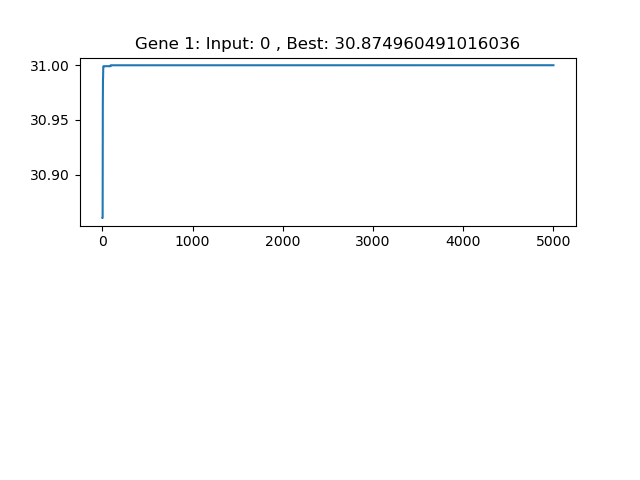
\includegraphics[width=6.4in,height=2.65in]{./media/image5.png}
	\end{Center}
\end{figure}


%%%%%%%%%%%%%%%%%%%% Figure/Image No: 5 Ends here %%%%%%%%%%%%%%%%%%%%

\par

Best Fitness: 898.9999935912551\par

Best Chromosome: [30.87496049]\par


\vspace{\baselineskip}

\vspace{\baselineskip}

\vspace{\baselineskip}

\vspace{\baselineskip}

\vspace{\baselineskip}

\vspace{\baselineskip}

\vspace{\baselineskip}

\vspace{\baselineskip}

\vspace{\baselineskip}
\begin{Center}
{\fontsize{28pt}{33.6pt}\selectfont Q III\par}
\end{Center}\par

{\fontsize{14pt}{16.8pt}\selectfont III) Understand the working of Bucket Brigade Classifier[BBC] (discussed in Goldberg)\par}\par

{\fontsize{14pt}{16.8pt}\selectfont \uline{Bucket Brigade Classifier}\par}\par

Classifier systems in machine learning is useful to distinguish three levels of activity when looking at learning from the point of view of classifier systems: At the lowest level is the performance system. This is the part of the overall system that interacts directly with the environment. It is much like an expert system, though typically less domain-dependent. The performance systems we will be talking about are rule-based, as are most expert systems, but they are message-passing, highly standardized, and highly parallel. Rules of this kind are called classifiers. These Rules must be evaluated for their performance, and here is where we use BBC.\par

The third level of activity, the rule discovery system, is required because, even after the system has effectively evaluated millions of rules, it has tested only a minuscule portion of the plausibly useful rules. Selection of the best of that minuscule portion can give little confidence that the system has exhausted its possibilities for improvement; it is even possible that none of the rules it has examined is very good. The system must be able to generate new rules to replace the least useful rules currently in place. The rules could be generated at random (say by $"$ mutation$"$  operators) or by running through a predetermined enumeration, but such $"$ experience-independent$"$  procedures produce improvements much too slowly to be useful in realistic settings. Somehow the rule discovery procedure must be biased by the system’s accumulated experience. In the present context this becomes a matter of using experience to determine useful $"$ building blocks$"$  for rules; then new rules are generated by combining selected building blocks. Under this procedure the new rules are at least plausible in terms of system experience. (Note that a rule may be plausible without necessarily being useful of even correct.) The rule discovery system discussed here employs genetic algorithms.\par

{\fontsize{14pt}{16.8pt}\selectfont \uline{Terms}\par}\par

\begin{enumerate}
	\item Credit \par

Generally the rules in the performance system are of varying usefulness and some, or even most, of them may be incorrect. Somehow the system must evaluate the rules. This activity is often called credit assignment (or apportionment of credit); accordingly this level of the system will be called the credit assignment system. \par

	\item Strength of a rule \par

A classifier system uses groups of rules as the representation. The structure of the concept is modeled by the organization, variability, and distribution of strength among the rules. Because the members of a group compete to become active, the appropriate aspects of the representation are selected only when they are relevant in a given problem solving context. The modularity of the concept thereby makes it easier to use as well as easier to modify. Basically, strength of a rule tells if the rule is applicable to a particular/ given environment. \par

	\item Classifier 
\end{enumerate}\par

The starting point for this approach to machine learning is a set of rulebased systems suited to rule discovery algorithms. The rules must lend themselves to processes that extract and recombine $"$ building blocks$"$  from currently useful rules to form new rules, and the rules must interact simply and in a highly parallel fashion. Classifier systems are parallel, message-passing, rule-based systems wherein all rules have the same simple form. In the simplest version all messages are required to be of a fixed length over a specified alphabet, typically k-bit binary strings. The rules are in the usual condition/ action form. The condition part specifies what kinds of messages satisfy (activate) the rule and the action part specifies what message is to be sent when the rule is satisfied. A classifier system consists of four basic parts. \par

\begin{adjustwidth}{1.0in}{0.0in}
a. The input interface translates the current state of the environment into standard messages. For example, the input interface may use property detectors to set the bit values (1: the current state has the property, 0: it does not) at given positions in an incoming message. \par

\end{adjustwidth}

\begin{adjustwidth}{1.0in}{0.0in}
b. The classifiers, the rules used by the system, define the system’s procedures for processing messages. \par

\end{adjustwidth}

\begin{adjustwidth}{1.0in}{0.0in}
c. The message list contains all current messages (those generated by the input interface and those generated by satisfied rules). \par

\end{adjustwidth}

\begin{adjustwidth}{1.0in}{0.0in}
d. The output interface translates some messages into effects or actions, actions that modify the state of the environment.\par

\end{adjustwidth}

A classifier system’s basic execution cycle consists of the following steps:\par

Step 1: Add all messages from the input interface to the message list.\par

Step 2: Compare all messages on the message list to all conditions of all classifiers and record all matches (satisfied conditions). \par

Step 3: For each set of matches satisfying the condition part of some classifier, post the message specified by its action part to a list of new messages.\par

Step 4: Replace all messages on the message list by the list of new messages. \par

Step 5: Translate messages on the message list to requirements on the output interface, thereby producing the system’s current output. \par

Step 6: Return to Step 1. \par

Individual classifiers must have a simple, compact definition if they are to serve as appropriate grist for the learning mill; a complex, interpreted definition makes it difficult for the learning algorithm to find and exploit building blocks from which to construct new rules. The major technical hurdle in implementing this definition is that of providing a simple specification of the condition part of the rule. Each condition must specify exactly the set of messages that satisfies it. Though most large sets can be defined only by an explicit listing, there is one class of subsets in the message space that can be specified quite compactly, the hyperplanes in that space. Specifically, let 1, 0 be the set of possible k-bit messages; if we use $"$ $"$  as a $"$ don’t care$"$  symbol, then the set of hyperplanes can be designated by the set of all ternary strings of length k over the alphabet 1, 0, . For example, the string 1... designates the set of all messages that start with a 1, while the string 00... 0 specifies the set 00... 01, 00... 00 consisting of exactly two messages, and so on. It is easy to check whether a given message satisfies a condition. The condition and the message are matched position by position, and if the entries at all non- positions are identical, then the message satisfies the condition. The notation is extended by allowing any string c over 1, 0, to be prefixed by a $"$ -$"$  with the intended interpretation that -c is satisfied just in case no message satisfying c is present on the message list.\par

{\fontsize{14pt}{16.8pt}\selectfont \uline{Credit Appointment using BBC }\par}\par

The first major learning task facing any rule-based system operating in a complex environment is the credit assignment task. Somehow the performance system must determine both the rules responsible for its successes and the representativeness of the conditions encountered in attaining the successes.The task is difficult because overt rewards are rare in complex environments; the system’s behavior is mostly $"$ stage-setting$"$  that makes possible later successes. The problem is even more difficult for parallel systems, where only some of the rules active at a given time may be instrumental in attaining later success. An environment exhibiting perpetual novelty adds still another order of complexity. Under such conditions the performance system can never have an absolute assurance that any of its rules is $"$ correct.$"$  The perpetual novelty of the environment, combined with an always limited sampling of that environment, leaves a residue to uncertainty. Each rule in effect serves as a hypothesis that has been more or less confirmed. The bucket brigade algorithm is designed to solve the credit assignment problem for classifier systems. To implement the algorithm, each classifier is assigned a quantity called its strength. The bucket brigade algorithm adjusts the strength to reflect the classifier’s overall usefulness to the system. The strength is then used as the basis of a competition. Each time step, each satisfied classifier makes a bid based on its strength, and only the highest bidding classifiers get their messages on the message list for the next time step. It is worth recalling that there are no consistency requirements on posted messages; the message list can hold any set of messages, and any such set can direct further competition. The only point at which consistency enters is at the output interface. Here, different sets of messages may specify conflicting responses. Such conflicts are again resolved by competition. For example, the strengths of the classifiers advocating each response can be summed so that one of the conflicting actions is chosen with a probability proportional to the sum of its advocates. \par


\vspace{\baselineskip}

\vspace{\baselineskip}
The bidding process is specified as follows. Let s(C, t) be the strength of classifier C at time t. Two factors clearly bear on the bidding process: \par

\begin{enumerate}
	\item relevance to the current situation. \par

	\item past $"$ usefulness$"$ . 
\end{enumerate}\par


\vspace{\baselineskip}
Relevance is mostly a matter of the specificity of the rule’s condition part–a more specific condition satisfied by the current situation conveys more information about that situation. The rule’s strength is supposed to reflect its usefulness. In the simplest versions of the competition the bid is a product of these two factors, being 0 if the rule is irrelevant (condition not satisfied) or useless (strength 0), and being high when the rule is highly specific to the situation (detailed conditions satisfied) and well confirmed as useful (high strength). To implement this bidding procedure, we modify Step 3 of the basic execution cycle, \par

For each set of matches satisfying the condition part of classifier C, calculate a bid according to the following formula, \par

 \[ B \left( C, t \right)  = b \ast R \left( C \right) s \left( C, t \right)   \] \par

R(C) is the specificity, equal to the number of non- in the condition part of C divided by the length thereof. \par

b is a constant less then one. \par

The size of the bid determines the probability that the classifier posts its message (specified by the action part) to the new message list. (E.g., the probability that the classifier posts its message might decrease exponentially as the size of the bid decreases.) \par

The use of probability in the revised step assures that rules of lower strength sometimes get tested, thereby providing for the occasional testing of less favored and newly generated (lower strength) classifiers ($"$ hypotheses$"$ ). \par

The operation of the bucket brigade algorithm can be explained informally via an economic analogy. The algorithm treats each rule as a kind of $"$ middleman$"$  in a complex economy. As a $"$ middleman,$"$  a rule only deals with its $"$ suppliers$"$ –the rules sending messages satisfying its conditions–and its $"$ consumers$"$ –the rules with conditions satisfied by the messages the $"$ middleman$"$  sends. Whenever a rule wins a bidding competition, it initiates a transaction wherein it pays out part of its strength to its suppliers. (If the rule does not bid enough to win the competition, it pays nothing.) As one of the winners of the competition, the rule becomes active, serving as a supplier to its consumers, and receiving payments from them in turn. Under this arrangement, the rule’s strength is a kind of capital that measures its ability to turn a $"$ profit.$"$  If a rule receives more from its consumers than it paid out, it has made a profit; that is, its strength has increased. \par

More formally, when a winning classifier C places its message on the message list it pays for the privilege by having its strength s(C, t) reduced by the amount of the bid B(C, t), \par

 \[ s \left( C, t + 1 \right)  = s \left( C, t \right)  - B \left( C, t \right)  \] \par

The Classifiers C’ sending messages matched by this winner, the $"$ suppliers,$"$  have their strengths increased by the amount of the bid–it is shared among them in the simplest version \par

 \[ s \left( C 0 , t + 1 \right)  = s \left( C 0 , t \right)  + aB \left( C, t \right)  \] \par

a =  \( \frac{1}{ \left(  \vert C^{'} \vert  \right) } \) \par


\vspace{\baselineskip}
A rule is likely to be profitable only if its consumers, in their local transactions, are also (on the average) profitable. The consumers, in turn, will be profitable only if their consumers are profitable. The resulting chains of consumers lead to the ultimate consumers, the rules that directly attain goals and receive payoff directly from the environment. (Payoff is added to the strengths of all rules determining responses at the time the payoff occurs.) A rule that regularly attains payoff when activated is of course profitable. The profitability of other rules depends upon their being coupled into sequences leading to these profitable ultimate consumers. The bucket brigade ensures that early acting, $"$ stage-setting$"$  rules eventually receive credit if they are coupled into (correlated with) sequences that (on average) lead to payoff. If a rule sequence is faulty, the final rule in the sequence loses strength, and the sequence will begin to disintegrate, over time, from the final rule backwards through its chain of precursors. As soon as a rule’s strength decreases to the point that it loses in the bidding process, some competing rule will get a chance to act as a replacement. If the competing rule is more useful than the one displaced, a revised rule sequence will begin to form using the new rule. The bucket brigade algorithm thus searches out and repairs $"$ weak links$"$  through its pervasive local application. Whenever rules are coupled into larger hierarchical knowledge structures, the bucket brigade algorithm is still more powerful than the description so far would suggest. Consider an abstract rule C$\ast$  of the general form, $"$ if the goal is G, and if the procedure P is executed, then G will be achieved.$"$  C$\ast$  will be active throughout the time interval in which the sequence of rules comprising P is executed. If the goal is indeed achieved, this rule serves to activate the response that attains the goal, as well as the stage-setting responses preceding that response. Under the bucket brigade C$\ast$  will be strengthened immediately by the goal attainment. On the very next trial involving P, the earliest rules in P will have their strengths substantially increased under the bucket brigade. This happens because the early rules act as suppliers to the strengthened C$\ast$  (via the condition $"$ if the procedure P is executed$"$ ). Normally, the process would have to be executed on the order of n times to back chain strength through an n-step process P. C$\ast$  circumvents this necessity.\par


\vspace{\baselineskip}

\vspace{\baselineskip}

\vspace{\baselineskip}

\vspace{\baselineskip}

\vspace{\baselineskip}

\vspace{\baselineskip}

\vspace{\baselineskip}

\vspace{\baselineskip}

\vspace{\baselineskip}

\vspace{\baselineskip}

\vspace{\baselineskip}

\vspace{\baselineskip}
\begin{Center}
{\fontsize{28pt}{33.6pt}\selectfont Q V\par}
\end{Center}\par

{\fontsize{14pt}{16.8pt}\selectfont V) Understand confusion matrix and various performance measures associated with classification tasks such as accuracy, sensitivity, specificity, precision, recall, F1 score etc. Consider a sample binary classifier results (TP, FP, TN, FN) and compute various measures.\par}\par

{\fontsize{14pt}{16.8pt}\selectfont \uline{Confusion Matrix}\par}\par

A confusion matrix is a summary of predicted results on a classification problem \par

Terms,\par

\begin{enumerate}
	\item Positive (P): outcome/observation is positive (Eg. it is a dog)\par

	\item Negative (N): outcome/observation is not positive (Eg. it is not a dog)\par

	\item True Positive (TP): prediction and observation are positive\par

	\item False Positive (FP): prediction is positive, but true observation is negative \par

	\item False Negative (FN): prediction is negative, but true observation is positive\par

	\item True Negative (TN): prediction and observation are not positive
\end{enumerate}\par

Formulas,\par

\begin{enumerate}
	\item Recall =  \( \frac{TP}{TP+FN} \)  (Also called sensitivity)\par

High Recall means the recognized class is correct\par

Low Recall means the recognized class is wrong\par


\vspace{\baselineskip}
	\item Precision =  \( \frac{TP}{TP+FP} \) \par

High Precision means if outcome is positive, in reality also it is positive\par

	\item Specificity =  \( \frac{TN}{TN+FN} \) \par

High Specificity means if outcome is negative, in reality also it is negative\par


\vspace{\baselineskip}
	\item Accuracy =  \( \frac{TP+TN}{TP+TN+FP+FN} \) \par


\vspace{\baselineskip}
	\item F1 Score =  \( \frac{2\astPrecision\astRecall}{Precision+Recall} \) 
\end{enumerate}\par


\vspace{\baselineskip}

\vspace{\baselineskip}
\begin{Center}
{\fontsize{28pt}{33.6pt}\selectfont Q VI\par}
\end{Center}\par

{\fontsize{14pt}{16.8pt}\selectfont VI) Clustering Algorithms (Euclidean distance may be used)\par}\par

\begin{enumerate}
	\item {\fontsize{14pt}{16.8pt}\selectfont Understand the working of k-means clustering algorithm. Give a pseudo code for the same and trace it for a sample dataset of your choice, clearly showing the centroid updates.\par}\par

{\fontsize{14pt}{16.8pt}\selectfont \uline{Pseudo Code}\par}\par

\begin{enumerate}
	\item {\fontsize{14pt}{16.8pt}\selectfont Choose random K Samples (initial centroid)\par}\par

	\item {\fontsize{14pt}{16.8pt}\selectfont For specified no of iterations, \par}\par

\begin{enumerate}
	\item {\fontsize{14pt}{16.8pt}\selectfont Form k clusters by assigning items to their closest mean/centroid\par}\par

	\item {\fontsize{14pt}{16.8pt}\selectfont Update the mean points by taking mean of each cluster\par}\par

	\item {\fontsize{14pt}{16.8pt}\selectfont Repeat\par}
\end{enumerate}
\end{enumerate}\par

{\fontsize{14pt}{16.8pt}\selectfont \uline{Trace}\par}\par

{\fontsize{14pt}{16.8pt}\selectfont Dataset\par}\par



%%%%%%%%%%%%%%%%%%%% Table No: 5 starts here %%%%%%%%%%%%%%%%%%%%


\begin{table}[H]
 			\centering
\begin{tabular}{p{1.96in}p{1.96in}p{1.96in}}
\hline
%row no:1
\multicolumn{1}{|p{1.96in}}{} & 
\multicolumn{1}{|p{1.96in}}{\Centering {\fontsize{14pt}{16.8pt}\selectfont X}} & 
\multicolumn{1}{|p{1.96in}|}{\Centering {\fontsize{14pt}{16.8pt}\selectfont Y}} \\
\hhline{---}
%row no:2
\multicolumn{1}{|p{1.96in}}{\Centering {\fontsize{14pt}{16.8pt}\selectfont 0}} & 
\multicolumn{1}{|p{1.96in}}{\Centering {\fontsize{14pt}{16.8pt}\selectfont 3}} & 
\multicolumn{1}{|p{1.96in}|}{\Centering {\fontsize{14pt}{16.8pt}\selectfont 4}} \\
\hhline{---}
%row no:3
\multicolumn{1}{|p{1.96in}}{\Centering {\fontsize{14pt}{16.8pt}\selectfont 1}} & 
\multicolumn{1}{|p{1.96in}}{\Centering {\fontsize{14pt}{16.8pt}\selectfont 7}} & 
\multicolumn{1}{|p{1.96in}|}{\Centering {\fontsize{14pt}{16.8pt}\selectfont 5}} \\
\hhline{---}
%row no:4
\multicolumn{1}{|p{1.96in}}{\Centering {\fontsize{14pt}{16.8pt}\selectfont 2}} & 
\multicolumn{1}{|p{1.96in}}{\Centering {\fontsize{14pt}{16.8pt}\selectfont 2}} & 
\multicolumn{1}{|p{1.96in}|}{\Centering {\fontsize{14pt}{16.8pt}\selectfont 6}} \\
\hhline{---}
%row no:5
\multicolumn{1}{|p{1.96in}}{\Centering {\fontsize{14pt}{16.8pt}\selectfont 3}} & 
\multicolumn{1}{|p{1.96in}}{\Centering {\fontsize{14pt}{16.8pt}\selectfont 3}} & 
\multicolumn{1}{|p{1.96in}|}{\Centering {\fontsize{14pt}{16.8pt}\selectfont 1}} \\
\hhline{---}
%row no:6
\multicolumn{1}{|p{1.96in}}{\Centering {\fontsize{14pt}{16.8pt}\selectfont 4}} & 
\multicolumn{1}{|p{1.96in}}{\Centering {\fontsize{14pt}{16.8pt}\selectfont 8}} & 
\multicolumn{1}{|p{1.96in}|}{\Centering {\fontsize{14pt}{16.8pt}\selectfont 2}} \\
\hhline{---}
%row no:7
\multicolumn{1}{|p{1.96in}}{\Centering {\fontsize{14pt}{16.8pt}\selectfont 5}} & 
\multicolumn{1}{|p{1.96in}}{\Centering {\fontsize{14pt}{16.8pt}\selectfont 7}} & 
\multicolumn{1}{|p{1.96in}|}{\Centering {\fontsize{14pt}{16.8pt}\selectfont 3}} \\
\hhline{---}
%row no:8
\multicolumn{1}{|p{1.96in}}{\Centering {\fontsize{14pt}{16.8pt}\selectfont 6}} & 
\multicolumn{1}{|p{1.96in}}{\Centering {\fontsize{14pt}{16.8pt}\selectfont 4}} & 
\multicolumn{1}{|p{1.96in}|}{\Centering {\fontsize{14pt}{16.8pt}\selectfont 4}} \\
\hhline{---}
%row no:9
\multicolumn{1}{|p{1.96in}}{\Centering {\fontsize{14pt}{16.8pt}\selectfont 7}} & 
\multicolumn{1}{|p{1.96in}}{\Centering {\fontsize{14pt}{16.8pt}\selectfont 6}} & 
\multicolumn{1}{|p{1.96in}|}{\Centering {\fontsize{14pt}{16.8pt}\selectfont 6}} \\
\hhline{---}
%row no:10
\multicolumn{1}{|p{1.96in}}{\Centering {\fontsize{14pt}{16.8pt}\selectfont 8}} & 
\multicolumn{1}{|p{1.96in}}{\Centering {\fontsize{14pt}{16.8pt}\selectfont 7}} & 
\multicolumn{1}{|p{1.96in}|}{\Centering {\fontsize{14pt}{16.8pt}\selectfont 4}} \\
\hhline{---}
%row no:11
\multicolumn{1}{|p{1.96in}}{\Centering {\fontsize{14pt}{16.8pt}\selectfont 9}} & 
\multicolumn{1}{|p{1.96in}}{\Centering {\fontsize{14pt}{16.8pt}\selectfont 6}} & 
\multicolumn{1}{|p{1.96in}|}{\Centering {\fontsize{14pt}{16.8pt}\selectfont 7}} \\
\hhline{---}

\end{tabular}
 \end{table}


%%%%%%%%%%%%%%%%%%%% Table No: 5 ends here %%%%%%%%%%%%%%%%%%%%


\vspace{\baselineskip}
{\fontsize{14pt}{16.8pt}\selectfont Choose random K = 2 means, \par}\par

{\fontsize{14pt}{16.8pt}\selectfont Let they be C1 – (1, 1) and C2 – (7, 7)\par}\par

{\fontsize{14pt}{16.8pt}\selectfont Each item is assigned to whichever cluster has least distance\par}\par

{\fontsize{14pt}{16.8pt}\selectfont So, C1 – 0, 2, 3, 6, \tab \tab and \tab C2 – 1, 4, 5, 7, 8, 9\par}\par

{\fontsize{14pt}{16.8pt}\selectfont Now find new mean of the clusters\par}\par

{\fontsize{14pt}{16.8pt}\selectfont C1(new) = ((3+2+3+4) / 4\  ,\  (4+6+1+4) / 4) = (3, 3.75)\par}\par

{\fontsize{14pt}{16.8pt}\selectfont C2(new) = ((7+8+7+6+7+6) / 6\  ,\  (5+2+3+6+4+7) / 6) = (6.83, 4.5)\par}\par

{\fontsize{14pt}{16.8pt}\selectfont Thus, means has been updated\par}\par

{\fontsize{14pt}{16.8pt}\selectfont Now, Repeat same process\par}\par


\vspace{\baselineskip}
	\item {\fontsize{14pt}{16.8pt}\selectfont Understand the working of k-medoids clustering algorithm. Give a pseudo code for the same and trace it for the sample dataset used for VI-(a), clearly showing the centroid updates. \par}\par

{\fontsize{14pt}{16.8pt}\selectfont \uline{Pseudo Code}\par}\par

\begin{enumerate}
	\item {\fontsize{14pt}{16.8pt}\selectfont Choose random K items from the given dataset (initial medoids)\par}\par

	\item {\fontsize{14pt}{16.8pt}\selectfont For specified no of iterations,\par}\par

\begin{enumerate}
	\item {\fontsize{14pt}{16.8pt}\selectfont Form k clusters by assigning items to their closest medoid\par}\par

	\item {\fontsize{14pt}{16.8pt}\selectfont Calculate the total dissimilarity\par}\par

	\item {\fontsize{14pt}{16.8pt}\selectfont Now, select a random non-medoid item as medoid and repeat (a) and (b)\par}\par

	\item {\fontsize{14pt}{16.8pt}\selectfont If cost/total dissimilarity is more for previous set of medoids than for the new medoid, then replace the old set with new set of medoid and Repeat from (a)\par}\par

	\item {\fontsize{14pt}{16.8pt}\selectfont If cost/total dissimilarity is more for new set of medoids than for the previous medoid, then rollback and keep the old set of medoid and Repeat (c)\par}
\end{enumerate}
\end{enumerate}\par

{\fontsize{14pt}{16.8pt}\selectfont \uline{Trace}\par}\par

{\fontsize{14pt}{16.8pt}\selectfont Dataset\par}\par



%%%%%%%%%%%%%%%%%%%% Table No: 6 starts here %%%%%%%%%%%%%%%%%%%%


\begin{table}[H]
 			\centering
\begin{tabular}{p{1.96in}p{1.96in}p{1.96in}}
\hline
%row no:1
\multicolumn{1}{|p{1.96in}}{} & 
\multicolumn{1}{|p{1.96in}}{\Centering {\fontsize{14pt}{16.8pt}\selectfont X}} & 
\multicolumn{1}{|p{1.96in}|}{\Centering {\fontsize{14pt}{16.8pt}\selectfont Y}} \\
\hhline{---}
%row no:2
\multicolumn{1}{|p{1.96in}}{\Centering {\fontsize{14pt}{16.8pt}\selectfont 0}} & 
\multicolumn{1}{|p{1.96in}}{\Centering {\fontsize{14pt}{16.8pt}\selectfont 3}} & 
\multicolumn{1}{|p{1.96in}|}{\Centering {\fontsize{14pt}{16.8pt}\selectfont 4}} \\
\hhline{---}
%row no:3
\multicolumn{1}{|p{1.96in}}{\Centering {\fontsize{14pt}{16.8pt}\selectfont 1}} & 
\multicolumn{1}{|p{1.96in}}{\Centering {\fontsize{14pt}{16.8pt}\selectfont 7}} & 
\multicolumn{1}{|p{1.96in}|}{\Centering {\fontsize{14pt}{16.8pt}\selectfont 5}} \\
\hhline{---}
%row no:4
\multicolumn{1}{|p{1.96in}}{\Centering {\fontsize{14pt}{16.8pt}\selectfont 2}} & 
\multicolumn{1}{|p{1.96in}}{\Centering {\fontsize{14pt}{16.8pt}\selectfont 2}} & 
\multicolumn{1}{|p{1.96in}|}{\Centering {\fontsize{14pt}{16.8pt}\selectfont 6}} \\
\hhline{---}
%row no:5
\multicolumn{1}{|p{1.96in}}{\Centering {\fontsize{14pt}{16.8pt}\selectfont 3}} & 
\multicolumn{1}{|p{1.96in}}{\Centering {\fontsize{14pt}{16.8pt}\selectfont 3}} & 
\multicolumn{1}{|p{1.96in}|}{\Centering {\fontsize{14pt}{16.8pt}\selectfont 1}} \\
\hhline{---}
%row no:6
\multicolumn{1}{|p{1.96in}}{\Centering {\fontsize{14pt}{16.8pt}\selectfont 4}} & 
\multicolumn{1}{|p{1.96in}}{\Centering {\fontsize{14pt}{16.8pt}\selectfont 8}} & 
\multicolumn{1}{|p{1.96in}|}{\Centering {\fontsize{14pt}{16.8pt}\selectfont 2}} \\
\hhline{---}
%row no:7
\multicolumn{1}{|p{1.96in}}{\Centering {\fontsize{14pt}{16.8pt}\selectfont 5}} & 
\multicolumn{1}{|p{1.96in}}{\Centering {\fontsize{14pt}{16.8pt}\selectfont 7}} & 
\multicolumn{1}{|p{1.96in}|}{\Centering {\fontsize{14pt}{16.8pt}\selectfont 3}} \\
\hhline{---}
%row no:8
\multicolumn{1}{|p{1.96in}}{\Centering {\fontsize{14pt}{16.8pt}\selectfont 6}} & 
\multicolumn{1}{|p{1.96in}}{\Centering {\fontsize{14pt}{16.8pt}\selectfont 4}} & 
\multicolumn{1}{|p{1.96in}|}{\Centering {\fontsize{14pt}{16.8pt}\selectfont 4}} \\
\hhline{---}
%row no:9
\multicolumn{1}{|p{1.96in}}{\Centering {\fontsize{14pt}{16.8pt}\selectfont 7}} & 
\multicolumn{1}{|p{1.96in}}{\Centering {\fontsize{14pt}{16.8pt}\selectfont 6}} & 
\multicolumn{1}{|p{1.96in}|}{\Centering {\fontsize{14pt}{16.8pt}\selectfont 6}} \\
\hhline{---}
%row no:10
\multicolumn{1}{|p{1.96in}}{\Centering {\fontsize{14pt}{16.8pt}\selectfont 8}} & 
\multicolumn{1}{|p{1.96in}}{\Centering {\fontsize{14pt}{16.8pt}\selectfont 7}} & 
\multicolumn{1}{|p{1.96in}|}{\Centering {\fontsize{14pt}{16.8pt}\selectfont 4}} \\
\hhline{---}
%row no:11
\multicolumn{1}{|p{1.96in}}{\Centering {\fontsize{14pt}{16.8pt}\selectfont 9}} & 
\multicolumn{1}{|p{1.96in}}{\Centering {\fontsize{14pt}{16.8pt}\selectfont 6}} & 
\multicolumn{1}{|p{1.96in}|}{\Centering {\fontsize{14pt}{16.8pt}\selectfont 7}} \\
\hhline{---}

\end{tabular}
 \end{table}


%%%%%%%%%%%%%%%%%%%% Table No: 6 ends here %%%%%%%%%%%%%%%%%%%%


\vspace{\baselineskip}
{\fontsize{14pt}{16.8pt}\selectfont Choose random K = 2 medoids, \par}\par

{\fontsize{14pt}{16.8pt}\selectfont Let they be C1 – (3, 1) (I3) and C2 – (6, 6) (I7)\par}\par

{\fontsize{14pt}{16.8pt}\selectfont Each item is assigned to whichever cluster has least dissimilarity\par}\par

{\fontsize{14pt}{16.8pt}\selectfont So, C1 – 0, 4, 6\tab and \tab C2 – 1, 2, 5, 8, 9\par}\par

{\fontsize{14pt}{16.8pt}\selectfont Total Diss = (3 + 6 + 4) + (2 + 4 + 4 + 3 + 1) = 13 + 14 = 27\par}\par

{\fontsize{14pt}{16.8pt}\selectfont Now, we choose randomly, (I8) = (7, 4) as medoid\par}\par

{\fontsize{14pt}{16.8pt}\selectfont C1 – (3, 1) and C2 – (7, 4)\par}\par

{\fontsize{14pt}{16.8pt}\selectfont Now,\ assignment\ is,\ C1\ – 0, 2     \tab and \tab C2 – 1, 4, 5, 6, 7, 9\par}\par

{\fontsize{14pt}{16.8pt}\selectfont Total Diss = (3 + 6) + (1 + 3 + 1 + 3 + 3 + 4) = 9 + 15 = 24\par}\par

{\fontsize{14pt}{16.8pt}\selectfont As 24 < 27, we change medoids to new set – C1 – (3, 1) and C2 – (7, 4)\par}\par

{\fontsize{14pt}{16.8pt}\selectfont Repeat above process\par}\par


\vspace{\baselineskip}
	\item {\fontsize{14pt}{16.8pt}\selectfont Understand the working of hierarchical clustering algorithm- Agglomerative, Divisive and trace them for the dataset used in VI-(a). You may trace the algorithm for both the approaches and use the dendrogram to represent the clustering process pictorially as well.\par}
\end{enumerate}\par

{\fontsize{14pt}{16.8pt}\selectfont \uline{Trace}\par}\par

{\fontsize{14pt}{16.8pt}\selectfont Agglomerative Clustering\par}\par

{\fontsize{14pt}{16.8pt}\selectfont Dataset\par}\par



%%%%%%%%%%%%%%%%%%%% Table No: 7 starts here %%%%%%%%%%%%%%%%%%%%


\begin{table}[H]
 			\centering
\begin{tabular}{p{1.96in}p{1.96in}p{1.96in}}
\hline
%row no:1
\multicolumn{1}{|p{1.96in}}{} & 
\multicolumn{1}{|p{1.96in}}{\Centering {\fontsize{14pt}{16.8pt}\selectfont X}} & 
\multicolumn{1}{|p{1.96in}|}{\Centering {\fontsize{14pt}{16.8pt}\selectfont Y}} \\
\hhline{---}
%row no:2
\multicolumn{1}{|p{1.96in}}{\Centering {\fontsize{14pt}{16.8pt}\selectfont 0}} & 
\multicolumn{1}{|p{1.96in}}{\Centering {\fontsize{14pt}{16.8pt}\selectfont 3}} & 
\multicolumn{1}{|p{1.96in}|}{\Centering {\fontsize{14pt}{16.8pt}\selectfont 4}} \\
\hhline{---}
%row no:3
\multicolumn{1}{|p{1.96in}}{\Centering {\fontsize{14pt}{16.8pt}\selectfont 1}} & 
\multicolumn{1}{|p{1.96in}}{\Centering {\fontsize{14pt}{16.8pt}\selectfont 7}} & 
\multicolumn{1}{|p{1.96in}|}{\Centering {\fontsize{14pt}{16.8pt}\selectfont 5}} \\
\hhline{---}
%row no:4
\multicolumn{1}{|p{1.96in}}{\Centering {\fontsize{14pt}{16.8pt}\selectfont 2}} & 
\multicolumn{1}{|p{1.96in}}{\Centering {\fontsize{14pt}{16.8pt}\selectfont 2}} & 
\multicolumn{1}{|p{1.96in}|}{\Centering {\fontsize{14pt}{16.8pt}\selectfont 6}} \\
\hhline{---}
%row no:5
\multicolumn{1}{|p{1.96in}}{\Centering {\fontsize{14pt}{16.8pt}\selectfont 3}} & 
\multicolumn{1}{|p{1.96in}}{\Centering {\fontsize{14pt}{16.8pt}\selectfont 3}} & 
\multicolumn{1}{|p{1.96in}|}{\Centering {\fontsize{14pt}{16.8pt}\selectfont 1}} \\
\hhline{---}
%row no:6
\multicolumn{1}{|p{1.96in}}{\Centering {\fontsize{14pt}{16.8pt}\selectfont 4}} & 
\multicolumn{1}{|p{1.96in}}{\Centering {\fontsize{14pt}{16.8pt}\selectfont 8}} & 
\multicolumn{1}{|p{1.96in}|}{\Centering {\fontsize{14pt}{16.8pt}\selectfont 2}} \\
\hhline{---}
%row no:7
\multicolumn{1}{|p{1.96in}}{\Centering {\fontsize{14pt}{16.8pt}\selectfont 5}} & 
\multicolumn{1}{|p{1.96in}}{\Centering {\fontsize{14pt}{16.8pt}\selectfont 7}} & 
\multicolumn{1}{|p{1.96in}|}{\Centering {\fontsize{14pt}{16.8pt}\selectfont 3}} \\
\hhline{---}
%row no:8
\multicolumn{1}{|p{1.96in}}{\Centering {\fontsize{14pt}{16.8pt}\selectfont 6}} & 
\multicolumn{1}{|p{1.96in}}{\Centering {\fontsize{14pt}{16.8pt}\selectfont 4}} & 
\multicolumn{1}{|p{1.96in}|}{\Centering {\fontsize{14pt}{16.8pt}\selectfont 4}} \\
\hhline{---}
%row no:9
\multicolumn{1}{|p{1.96in}}{\Centering {\fontsize{14pt}{16.8pt}\selectfont 7}} & 
\multicolumn{1}{|p{1.96in}}{\Centering {\fontsize{14pt}{16.8pt}\selectfont 6}} & 
\multicolumn{1}{|p{1.96in}|}{\Centering {\fontsize{14pt}{16.8pt}\selectfont 6}} \\
\hhline{---}
%row no:10
\multicolumn{1}{|p{1.96in}}{\Centering {\fontsize{14pt}{16.8pt}\selectfont 8}} & 
\multicolumn{1}{|p{1.96in}}{\Centering {\fontsize{14pt}{16.8pt}\selectfont 7}} & 
\multicolumn{1}{|p{1.96in}|}{\Centering {\fontsize{14pt}{16.8pt}\selectfont 4}} \\
\hhline{---}
%row no:11
\multicolumn{1}{|p{1.96in}}{\Centering {\fontsize{14pt}{16.8pt}\selectfont 9}} & 
\multicolumn{1}{|p{1.96in}}{\Centering {\fontsize{14pt}{16.8pt}\selectfont 6}} & 
\multicolumn{1}{|p{1.96in}|}{\Centering {\fontsize{14pt}{16.8pt}\selectfont 7}} \\
\hhline{---}

\end{tabular}
 \end{table}


%%%%%%%%%%%%%%%%%%%% Table No: 7 ends here %%%%%%%%%%%%%%%%%%%%


\vspace{\baselineskip}
{\fontsize{14pt}{16.8pt}\selectfont Initially, every item is a cluster – C0, C1, $ \ldots $  C9\par}\par



%%%%%%%%%%%%%%%%%%%% Figure/Image No: 6 starts here %%%%%%%%%%%%%%%%%%%%

\begin{figure}[H]
	\begin{Center}
		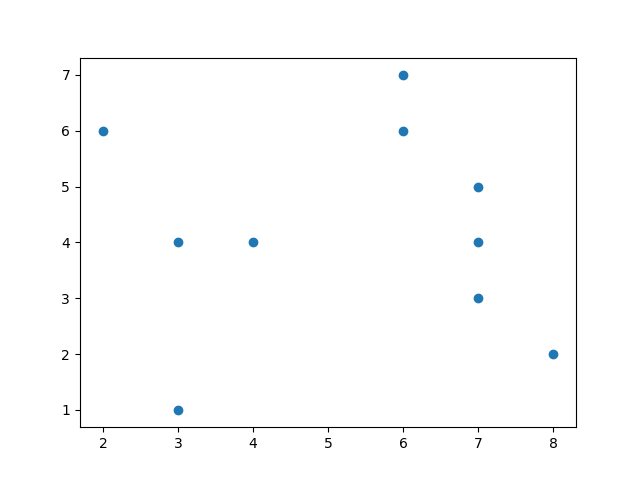
\includegraphics[width=6.4in,height=4.8in]{./media/image6.png}
	\end{Center}
\end{figure}


%%%%%%%%%%%%%%%%%%%% Figure/Image No: 6 Ends here %%%%%%%%%%%%%%%%%%%%

\par

{\fontsize{14pt}{16.8pt}\selectfont Closest 2 items are (3, 4) and (4, 4) (C0 and C6)\par}\par

{\fontsize{14pt}{16.8pt}\selectfont So, Merge them into 1 cluster C06 – (3.5, 4.0)\par}\par

{\fontsize{14pt}{16.8pt}\selectfont Next Closest 2 items are (7, 5) and (7, 4) (C1 and C8)\par}\par

{\fontsize{14pt}{16.8pt}\selectfont So, Merge them into 1 cluster C18 – (7.0, 4.5)\par}\par

{\fontsize{14pt}{16.8pt}\selectfont Simlarly merging, \par}\par

{\fontsize{14pt}{16.8pt}\selectfont Finally 3 Clusters\par}\par



%%%%%%%%%%%%%%%%%%%% Figure/Image No: 7 starts here %%%%%%%%%%%%%%%%%%%%

\begin{figure}[H]
	\begin{Center}
		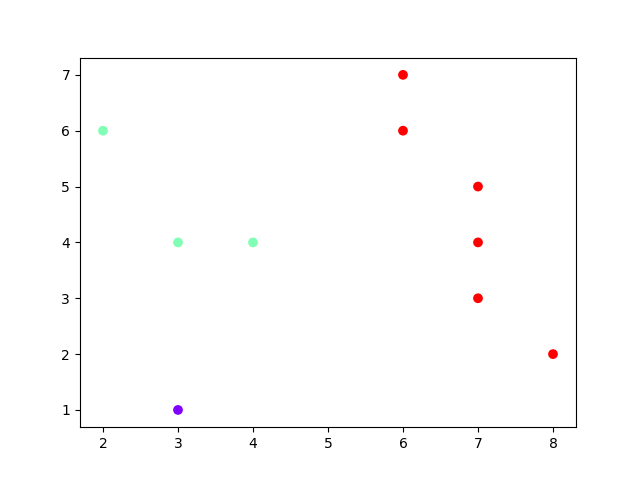
\includegraphics[width=6.4in,height=4.8in]{./media/image7.png}
	\end{Center}
\end{figure}


%%%%%%%%%%%%%%%%%%%% Figure/Image No: 7 Ends here %%%%%%%%%%%%%%%%%%%%

\par


\vspace{\baselineskip}

\vspace{\baselineskip}

\vspace{\baselineskip}

\vspace{\baselineskip}

\vspace{\baselineskip}

\vspace{\baselineskip}

\vspace{\baselineskip}

\vspace{\baselineskip}
\begin{Center}
{\fontsize{28pt}{33.6pt}\selectfont Q VII\par}
\end{Center}\par

{\fontsize{14pt}{16.8pt}\selectfont VII) Survey the various distance measures used by clustering algorithms eg: Cosine, Jaccard similarity measures etc.\par}\par

{\fontsize{14pt}{16.8pt}\selectfont Explore for a minimum of 5 measures (non-Euclidean distance measures) and trace them to measure distance 2 data points.\par}\par


\vspace{\baselineskip}
{\fontsize{14pt}{16.8pt}\selectfont \uline{Cosine Distance}\par}\par



%%%%%%%%%%%%%%%%%%%% Figure/Image No: 8 starts here %%%%%%%%%%%%%%%%%%%%

\begin{figure}[H]
	\begin{Center}
		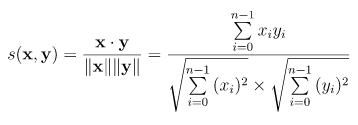
\includegraphics[width=3.73in,height=1.3in]{./media/image8.png}
	\end{Center}
\end{figure}


%%%%%%%%%%%%%%%%%%%% Figure/Image No: 8 Ends here %%%%%%%%%%%%%%%%%%%%

\par

{\fontsize{14pt}{16.8pt}\selectfont X = (2, 3)\par}\par

{\fontsize{14pt}{16.8pt}\selectfont Y = (4, 1)\par}\par

{\fontsize{14pt}{16.8pt}\selectfont Distance =  \( \frac{2\ast4+3\ast1}{\sqrt[]{2^{2}+ 3^{2}~}\ast \sqrt[]{4^{2}+ 1^{2}}} \) \  =  \( \frac{11}{\sqrt[]{13} \ast \sqrt[]{17}} \) \ \  =  \( \frac{11}{14.87} \) \ \  = 0.739\par}\par


\vspace{\baselineskip}

\vspace{\baselineskip}

\vspace{\baselineskip}
{\fontsize{14pt}{16.8pt}\selectfont \uline{Jaccard Distance}\par}\par



%%%%%%%%%%%%%%%%%%%% Figure/Image No: 9 starts here %%%%%%%%%%%%%%%%%%%%

\begin{figure}[H]
	\begin{Center}
		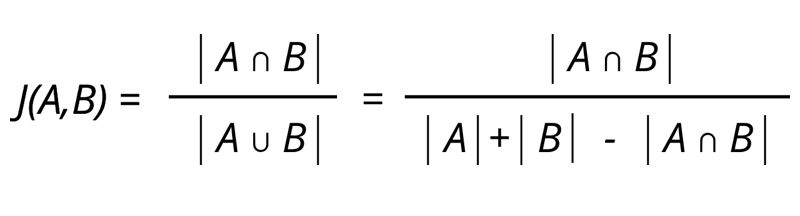
\includegraphics[width=3.67in,height=0.99in]{./media/image9.png}
	\end{Center}
\end{figure}


%%%%%%%%%%%%%%%%%%%% Figure/Image No: 9 Ends here %%%%%%%%%%%%%%%%%%%%

\par

{\fontsize{14pt}{16.8pt}\selectfont A = $ \{ $ 1, 2, 3, 4$ \} $ \par}\par

{\fontsize{14pt}{16.8pt}\selectfont B = $ \{ $ 1, 2$ \} $ \par}\par

{\fontsize{14pt}{16.8pt}\selectfont J(A, B) = 2 / 4 = 0.5\par}\par

{\fontsize{14pt}{16.8pt}\selectfont Jaccard Distance = 1 – Jaccard Similarity = 1 – 0.5 = 0.5\par}\par

{\fontsize{14pt}{16.8pt}\selectfont \uline{Manhattan Distance}\par}\par



%%%%%%%%%%%%%%%%%%%% Figure/Image No: 10 starts here %%%%%%%%%%%%%%%%%%%%

\begin{figure}[H]
	\begin{Center}
		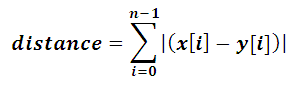
\includegraphics[width=3.13in,height=0.92in]{./media/image10.png}
	\end{Center}
\end{figure}


%%%%%%%%%%%%%%%%%%%% Figure/Image No: 10 Ends here %%%%%%%%%%%%%%%%%%%%

\par

{\fontsize{14pt}{16.8pt}\selectfont X = (4, 3)\par}\par

{\fontsize{14pt}{16.8pt}\selectfont Y = (8, 2)\par}\par

{\fontsize{14pt}{16.8pt}\selectfont Manhattan Distance = $ \vert $ (4 - 8)$ \vert $  + $ \vert $ (3 - 2)$ \vert $  = 4 + 1 = 5\par}\par

{\fontsize{14pt}{16.8pt}\selectfont \uline{Bray-Curtis Distance}\par}\par



%%%%%%%%%%%%%%%%%%%% Figure/Image No: 11 starts here %%%%%%%%%%%%%%%%%%%%

\begin{figure}[H]
	\begin{Center}
		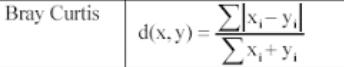
\includegraphics[width=3.58in,height=0.7in]{./media/image11.png}
	\end{Center}
\end{figure}


%%%%%%%%%%%%%%%%%%%% Figure/Image No: 11 Ends here %%%%%%%%%%%%%%%%%%%%

\par

{\fontsize{14pt}{16.8pt}\selectfont X = (3, 1)\par}\par

{\fontsize{14pt}{16.8pt}\selectfont Y = (7, 3)\par}\par

{\fontsize{14pt}{16.8pt}\selectfont Bray-Curtis Distance =  \( \frac{ \vert 3-7 \vert + \vert 1-3 \vert }{ \left( 3+7 \right) + \left( 1+3 \right) } \)  =  \( \frac{6}{14} \)  = 0.429\par}\par

{\fontsize{14pt}{16.8pt}\selectfont \uline{Chebychev Distance}\par}\par


\vspace{\baselineskip}


%%%%%%%%%%%%%%%%%%%% Figure/Image No: 12 starts here %%%%%%%%%%%%%%%%%%%%

\begin{figure}[H]
	\begin{Center}
		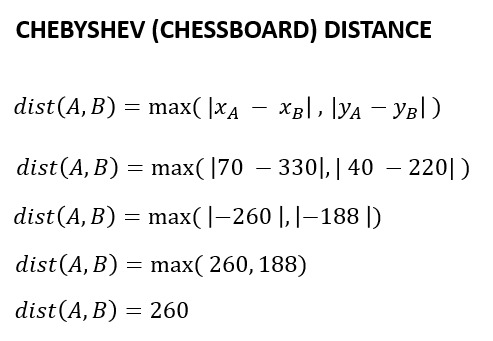
\includegraphics[width=5.13in,height=0.5in]{./media/image12.png}
	\end{Center}
\end{figure}


%%%%%%%%%%%%%%%%%%%% Figure/Image No: 12 Ends here %%%%%%%%%%%%%%%%%%%%

\par

{\fontsize{14pt}{16.8pt}\selectfont A = (3, 6)\par}\par

{\fontsize{14pt}{16.8pt}\selectfont B = (1, 7)\par}\par

{\fontsize{14pt}{16.8pt}\selectfont Chebychev Distance = max ($ \vert $ 3-1$ \vert $ , $ \vert $ 6-7$ \vert $ ) = max (2, 1) = 2\par}\par


\vspace{\baselineskip}

\vspace{\baselineskip}

\vspace{\baselineskip}
\begin{Center}
{\fontsize{28pt}{33.6pt}\selectfont Q VIII\par}
\end{Center}\par

{\fontsize{14pt}{16.8pt}\selectfont VIII) \par}\par

{\fontsize{14pt}{16.8pt}\selectfont a) Test drive/Implement Decision tree, Naive Bayes, BPN, k-means, hierarchical clustering in a platform of your choice.\par}\par

{\fontsize{14pt}{16.8pt}\selectfont \uline{Decision Tree}\par}\par



%%%%%%%%%%%%%%%%%%%% Figure/Image No: 13 starts here %%%%%%%%%%%%%%%%%%%%

\begin{figure}[H]
	\begin{Center}
		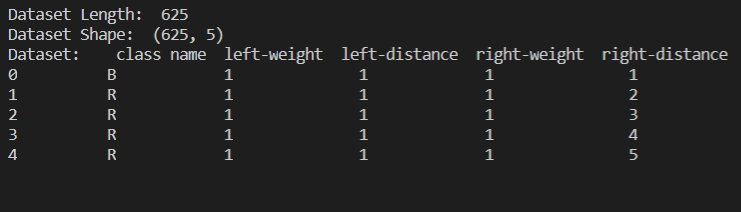
\includegraphics[width=6.5in,height=1.86in]{./media/image13.png}
	\end{Center}
\end{figure}


%%%%%%%%%%%%%%%%%%%% Figure/Image No: 13 Ends here %%%%%%%%%%%%%%%%%%%%

\par



%%%%%%%%%%%%%%%%%%%% Figure/Image No: 14 starts here %%%%%%%%%%%%%%%%%%%%

\begin{figure}[H]
	\begin{Center}
		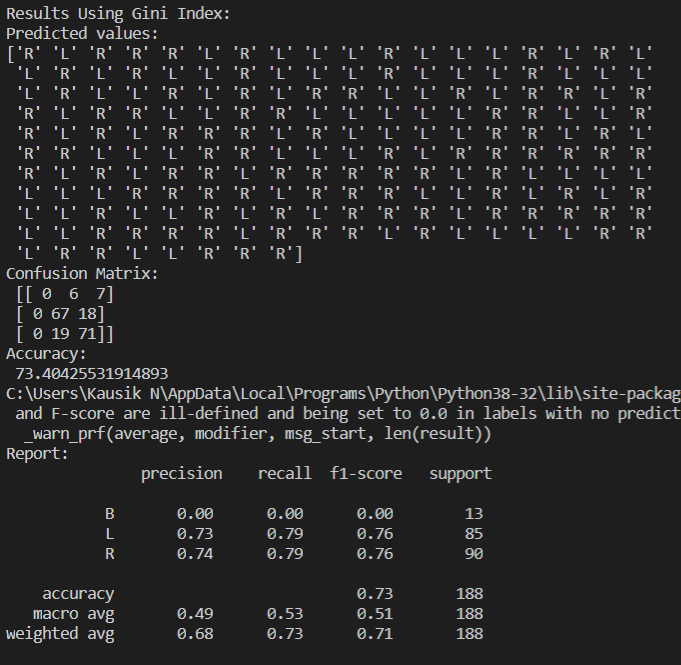
\includegraphics[width=6.5in,height=5.13in]{./media/image14.png}
	\end{Center}
\end{figure}


%%%%%%%%%%%%%%%%%%%% Figure/Image No: 14 Ends here %%%%%%%%%%%%%%%%%%%%

\par



%%%%%%%%%%%%%%%%%%%% Figure/Image No: 15 starts here %%%%%%%%%%%%%%%%%%%%

\begin{figure}[H]
	\begin{Center}
		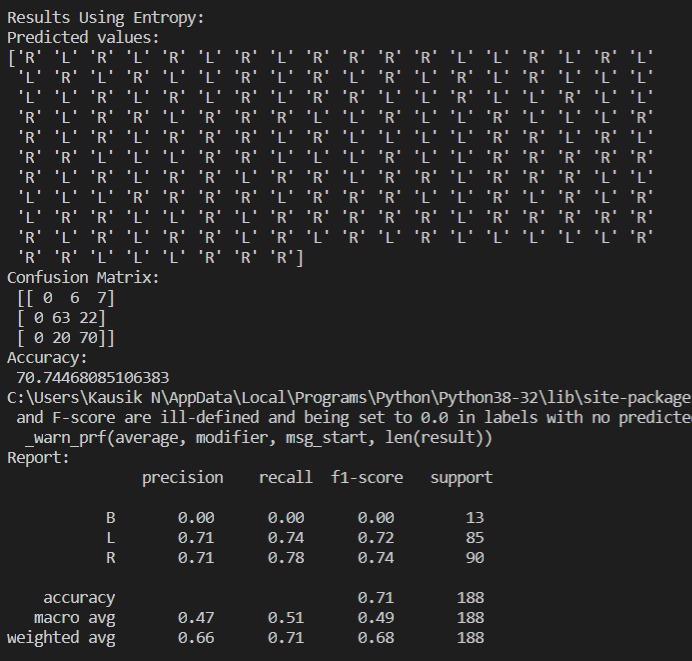
\includegraphics[width=6.5in,height=6.21in]{./media/image15.png}
	\end{Center}
\end{figure}


%%%%%%%%%%%%%%%%%%%% Figure/Image No: 15 Ends here %%%%%%%%%%%%%%%%%%%%

\par


\vspace{\baselineskip}

\vspace{\baselineskip}

\vspace{\baselineskip}

\vspace{\baselineskip}

\vspace{\baselineskip}

\vspace{\baselineskip}

\vspace{\baselineskip}

\vspace{\baselineskip}
{\fontsize{14pt}{16.8pt}\selectfont \uline{Naive Bayes Classifier}\par}\par

{\fontsize{14pt}{16.8pt}\selectfont Using Iris Dataset\par}\par



%%%%%%%%%%%%%%%%%%%% Figure/Image No: 16 starts here %%%%%%%%%%%%%%%%%%%%

\begin{figure}[H]
	\begin{Center}
		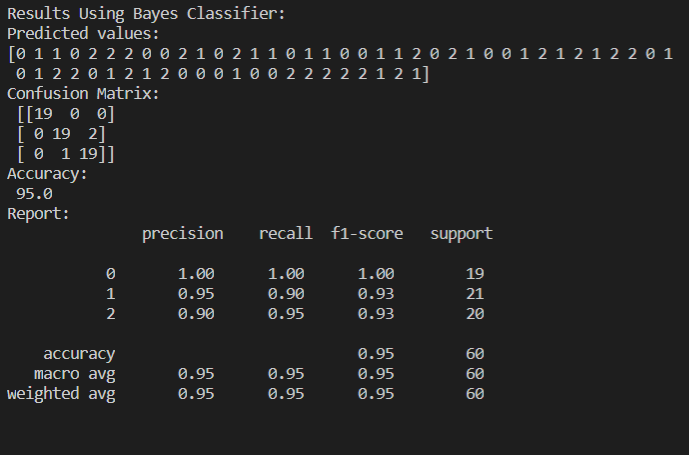
\includegraphics[width=6.5in,height=4.29in]{./media/image16.png}
	\end{Center}
\end{figure}


%%%%%%%%%%%%%%%%%%%% Figure/Image No: 16 Ends here %%%%%%%%%%%%%%%%%%%%

\par

{\fontsize{14pt}{16.8pt}\selectfont \uline{K-Means Clustering}\par}\par

{\fontsize{14pt}{16.8pt}\selectfont 100 Random Points between 0 to 100 values\par}\par



%%%%%%%%%%%%%%%%%%%% Figure/Image No: 17 starts here %%%%%%%%%%%%%%%%%%%%

\begin{figure}[H]
	\begin{Center}
		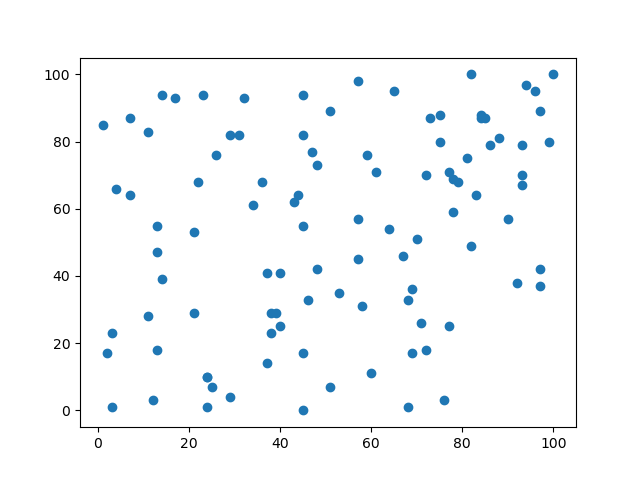
\includegraphics[width=6.4in,height=3.15in]{./media/image17.png}
	\end{Center}
\end{figure}


%%%%%%%%%%%%%%%%%%%% Figure/Image No: 17 Ends here %%%%%%%%%%%%%%%%%%%%

\par

{\fontsize{14pt}{16.8pt}\selectfont 3 Clusters\par}\par



%%%%%%%%%%%%%%%%%%%% Figure/Image No: 18 starts here %%%%%%%%%%%%%%%%%%%%

\begin{figure}[H]
	\begin{Center}
		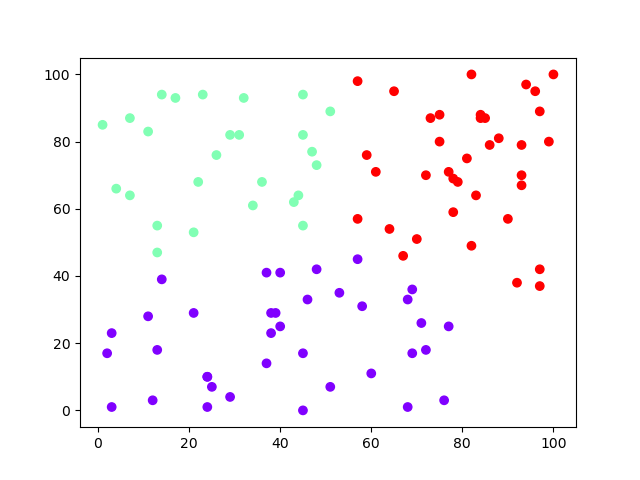
\includegraphics[width=6.4in,height=4.8in]{./media/image18.png}
	\end{Center}
\end{figure}


%%%%%%%%%%%%%%%%%%%% Figure/Image No: 18 Ends here %%%%%%%%%%%%%%%%%%%%

\par


\vspace{\baselineskip}

\vspace{\baselineskip}

\vspace{\baselineskip}

\vspace{\baselineskip}

\vspace{\baselineskip}

\vspace{\baselineskip}

\vspace{\baselineskip}

\vspace{\baselineskip}

\vspace{\baselineskip}

\vspace{\baselineskip}

\vspace{\baselineskip}
{\fontsize{14pt}{16.8pt}\selectfont \uline{Agglomerative Clustering}\par}\par

{\fontsize{14pt}{16.8pt}\selectfont 100 Random Points between 0 to 100\par}\par



%%%%%%%%%%%%%%%%%%%% Figure/Image No: 19 starts here %%%%%%%%%%%%%%%%%%%%

\begin{figure}[H]
	\begin{Center}
		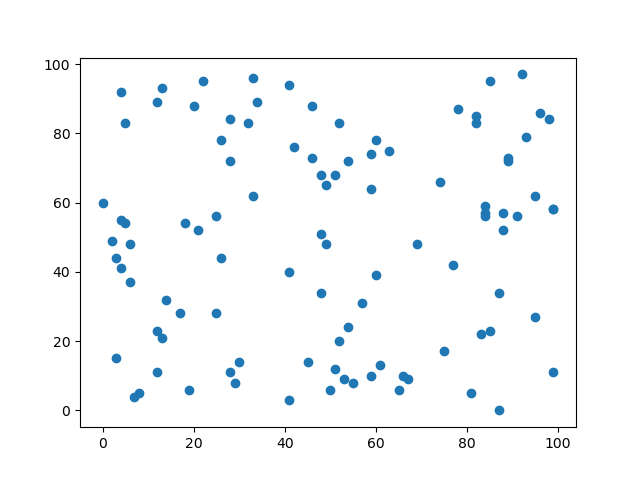
\includegraphics[width=6.4in,height=4.8in]{./media/image19.png}
	\end{Center}
\end{figure}


%%%%%%%%%%%%%%%%%%%% Figure/Image No: 19 Ends here %%%%%%%%%%%%%%%%%%%%

\par

{\fontsize{14pt}{16.8pt}\selectfont 3 Clusters\par}\par



%%%%%%%%%%%%%%%%%%%% Figure/Image No: 20 starts here %%%%%%%%%%%%%%%%%%%%

\begin{figure}[H]
	\begin{Center}
		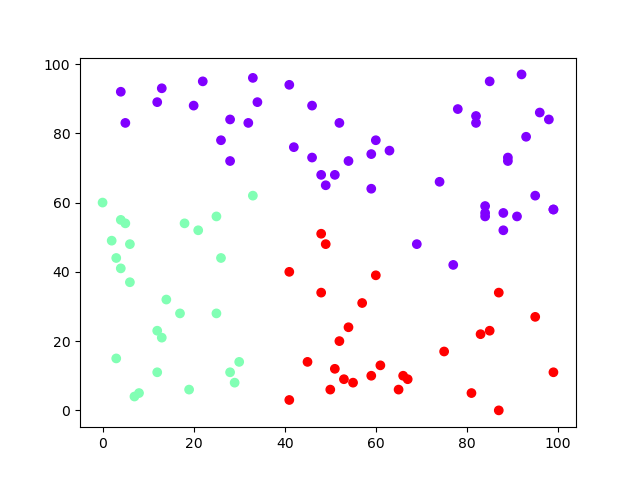
\includegraphics[width=6.4in,height=4.8in]{./media/image20.png}
	\end{Center}
\end{figure}


%%%%%%%%%%%%%%%%%%%% Figure/Image No: 20 Ends here %%%%%%%%%%%%%%%%%%%%

\par


\vspace{\baselineskip}
{\fontsize{14pt}{16.8pt}\selectfont b) Test drive/Implement optimization using GA operator in a platform of your choice (Not mandatory)\par}\par

{\fontsize{14pt}{16.8pt}\selectfont Inputs\par}\par

{\fontsize{10pt}{12.0pt}\selectfont \textcolor[HTML]{D4D4D4}{sol\_per\_pop = 200 $\#$  Defining the population size.}\par}\par

{\fontsize{10pt}{12.0pt}\selectfont \textcolor[HTML]{D4D4D4}{num\_generations = 5000}\par}\par

{\fontsize{10pt}{12.0pt}\selectfont \textcolor[HTML]{D4D4D4}{num\_parents\_mating = 100}\par}\par


\vspace{\baselineskip}
{\fontsize{10pt}{12.0pt}\selectfont \textcolor[HTML]{D4D4D4}{select\_mating\_pool = select\_mating\_pool\_bestfitness}\par}\par

{\fontsize{10pt}{12.0pt}\selectfont \textcolor[HTML]{D4D4D4}{crossover = crossover\_OnePoint}\par}\par

{\fontsize{10pt}{12.0pt}\selectfont \textcolor[HTML]{D4D4D4}{mutation = mutation\_UniformNoise}\par}\par

{\fontsize{10pt}{12.0pt}\selectfont \textcolor[HTML]{D4D4D4}{fitness\_func = PolyLinearFitness}\par}\par

{\fontsize{10pt}{12.0pt}\selectfont \textcolor[HTML]{D4D4D4}{boundary = (None, None)}\par}\par

{\fontsize{10pt}{12.0pt}\selectfont \textcolor[HTML]{D4D4D4}{equation\_inputs = [4, -2, 3.5, 5, -11, -4.7, 2.5, 0.1]}\par}\par

{\fontsize{10pt}{12.0pt}\selectfont \textcolor[HTML]{D4D4D4}{num\_weights = len(equation\_inputs) $\#$  Number of the weights we are looking to optimize.}\par}\par


\vspace{\baselineskip}

\vspace{\baselineskip}
{\fontsize{14pt}{16.8pt}\selectfont After Optimising,\par}\par

Best Fitness: 13920.720451463068\par

Best Chromosome: [ 411.87721227 -240.46700836\  384.55563335\  444.05949469 -501.41256815\par

 -415.91873926\  302.42510916\ \  16.55506078]\par

{\fontsize{10pt}{12.0pt}\selectfont Fitness Graph\par}\par



%%%%%%%%%%%%%%%%%%%% Figure/Image No: 21 starts here %%%%%%%%%%%%%%%%%%%%

\begin{figure}[H]
	\begin{Center}
		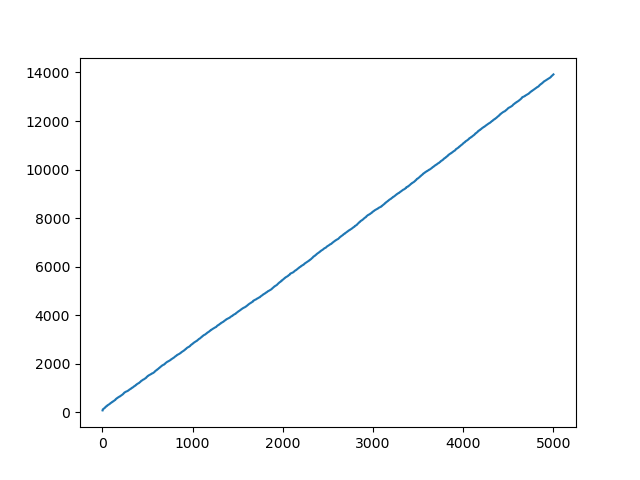
\includegraphics[width=3.45in,height=2.59in]{./media/image21.png}
	\end{Center}
\end{figure}


%%%%%%%%%%%%%%%%%%%% Figure/Image No: 21 Ends here %%%%%%%%%%%%%%%%%%%%

\par


\vspace{\baselineskip}
Gene Updation Graph\par

\par


\printbibliography
\end{document}